\chapter{\label{chap: spin-2}
Topological interfaces in spin-2 Bose-Einstein condensates}
In this chapter, we both analytically and numerically investigate the physics
of topological defects when connected across topological interfaces in spin-2
Bose-Einstein condensates.
We begin by introducing the concept of a topological interface, and discuss
systems where they can arise.
We then construct interpolating spinor wave functions for a spin-2 system that
smoothly connect states with different symmetries, forming a topological
interface.
Such interfaces include connections between the UN and BN phases, cyclic to both
nematic (UN/BN) phases, cyclic to FM phases, and also between the FM and BN
phases.
With these interpolating solutions, we then construct a rich phenomenology of
different defect states connecting across the interface.
These defects range from singular phase vortices, spin vortices, nonsingular
textures, and even to point defects such as monopoles.
Additionally, we also perform numerical simulations for select examples,
highlighting the interesting physics occurring at the interface.

\section{Introduction to topological interfaces}
Topological interfaces may form at the phase boundary between
topologically distinct phases that are described by different order parameters.
In such an interface, the phases can coexist in such a way that the different
symmetries connect smoothly across the boundary.
These interfaces arise in many areas of physics, such as in the context of
domain walls in the early universe~\cite{Zeldovich1975,Kibble1976,Kibble1980},
the \(A\)--\(B\) phase boundary in superfluid liquid \(^3\)He~\cite{
    Osheroff1977,Yip1986,Salomaa1987,Finne2006,Bradley2008,Volovik2009}, and in
atomic Bose-Einstein condensates (BECs)~\cite{Takeuchi2006,Kasamatsu2010,
    Borgh2012,Borgh2013, Borgh2014,Kaneda2014}.
When the order parameters on either side of the interface exhibit point-group
symmetries~\cite{Xiao2022}, families of vastly different defects
and textures may exist, where the topological charges of each defect depends
on other defects within the system~\cite{Poenaru1977, Mermin1979}.
An example is the cyclic and BN phases of spin-2 BECs, which, as we calculated
in Sec.~\ref{subsec: spin-2-homotopy}, have non-Abelian first homotopy groups,
and hence support non-Abelian defects whose topological charges do not commute.
Due to the different symmetries on either side of the interface, defects cannot
typically cross the interface unchanged.
Instead, the defect must either terminate at the boundary, or continuously
and non-trivially connect to an object representing a different topology on the
other side of the interface.

As shown in Chapter~\ref{chap: ground-states}, spin-1 and spin-2 systems offer a
rich ground state phase diagram with a myriad of different order parameter
symmetries.
In spin-1 systems, methods have already been proposed to engineer topological
interfaces between the different order parameter symmetries by use of Zeeman
shifts~\cite{Borgh2012, Borgh2013, Borgh2014}.
Naturally, since the spin-2 system offers even more choice of order parameter
symmetry, they make an excellent candidate for further investigating topological
interfaces.
Additionally, spinor BECs support wide family of topological defects exhibiting
different order parameter symmetries, cementing them as an ideal test bed
for connections of topological defects across such interfaces.
A small selection of vortices in the spin-2 system has already been considered
in Sec.~\ref{sec: vortices-spin-2}.
However, spin-2 systems support a much larger family of vortices and higher
order topological defects. 
These include, but are not limited to, integer vortices~\cite{Yip1999,
Isoshima2002,Mizushima2002,Sadler2006,Semenoff2007,Lovegrove2012,
Lovegrove2016,Borgh2016,Weiss2019,Xiao2021,Xiao2022}, vortices with fractional
charges~\cite{Leonhardt2000,Zhou2003,Ji2008,Seo2015,Semenoff2007,Kobayashi2009,
Lovegrove2012,Lovegrove2016,Borgh2016,Borgh2017,Xiao2021,Xiao2022}, nonsingular
vortices such as 2D Skyrmions~\cite{Ohmi1998, Ho1998, Mizushima2002a,
Martikainen2002, Leanhardt2003, Mizushima2004, Choi2012, Choi2012a,
Lovegrove2014,Weiss2019} and point defects such as monopoles~\cite{Stoof2001,
Savage2003,Ruostekoski2003,Pietila2009,Ray2014,Ray2015,Ollikainen2017,
Mithun2022,Blinova2023}.

\subsection{Engineering topological interfaces in spinor Bose-Einstein
condensates}
In a continuous spinor superfluid, it is possible for distinct phases with
varying order parameter symmetry to coexist.
A spinor BEC may be engineered such that separate regions of the condensate
have distinct ground state phases, e.g., nematic or cyclic, and hence have
different order parameter symmetries, creating a topological interface within
the condensate itself.
This can be achieved through variation of parameters in the Hamiltonian, such as
the linear and quadratic Zeeman shifts, which locally stabilise the different
regions.
If the parameter fluctuation is sufficiently acute, then the wave function will
interpolate between the bulk phases across a distance given by an appropriate
healing length.
In addition, as proposed for the spin-1 system~\cite{Borgh2014}, linear \(p\)
and quadratic \(q\) Zeeman shifts form the basis for engineering interpolating
solutions that model the topological interface.
Such steady-state solutions are found from the mean-field Hamiltonian density
functional discussed in Chapter~\ref{chap: theory} for a uniform system in the
presence of an external magnetic field using the relation \(\delta \mathcal{H}
/ \delta \zeta_m^*=0\)~\cite{Kawaguchi2012}:
\begin{equation}\label{eq: spin-2-GPEs-time-reversal}
    \left[-p \hat{F}_z + q \hat{F}^2_z + c_0n \, \zeta^\dagger \zeta
        + c_1n \, \langle\hat{\vb{F}}\rangle\cdot \vb{f}
        + \frac{c_2n}{5}{(\hat{\mathcal{T}}\zeta)}^\dagger \,
        \zeta\hat{\mathcal{T}} -\mu \right] \zeta = 0,
\end{equation}
where \(\mu \) is the chemical potential and \(\hat{\mathcal{T}}\) is a
time-reversal operator defined as \({(\hat{\mathcal{T}}\zeta)}_m =
{(-1)}^m\zeta_{-m}^*\).
Eq.~\eqref{eq: spin-2-GPEs-time-reversal} presents a non-linear system of
equations that can be solved for the unknown
\(\zeta_m\)~\cite{Ciobanu2000,Kawaguchi2012}.
Detailed derivations of each interpolating solution used in the subsequent
sections can be found in Appendix~\ref{appendix: stationary}.

Using the constructed interpolating stationary states, defect states for a given
spin-2 phase can, in principle, be constructed from
the representative spinor by defining an appropriate azimuthal phase winding,
\(\chi_m \), in each component, i.e., \(\text{Arg}(\zeta_m) =\chi_m =
k_m\varphi \), where \(k_m\) is an integer which denotes a generalisation to
multiple quantisation, and \(\varphi \) is the azimuthal angle around the vortex
core.
In addition, we also create a unitary framework which is applicable for
constructing other types of defect states across topological interfaces in a
spin-2 BEC, such as monopoles or nonsingular textures.
A given defect state can be constructed from the uniform interpolating state by
applying a global phase winding, \(\tau \), coupled with a spin rotation defined
by three Euler angles \((\alpha, \beta, \gamma)\) as in
Eq.~\eqref{eq: spin-2-rotation-matrix}.
When the same transformation is supported by two phases, A and B, of a spin-2
condensate, a general defect connection across an interface between the two
phases is given as
\begin{align}\label{eq: general-defect-interface}
    \zeta = e^{i\tau}\,U(\alpha, \beta, \gamma)\,\zeta^\text{A-B}.
\end{align}
Through the subsequent sections we provide various steady-state solutions that
interpolate between the different phases of a spin-2 BEC\@.
Using these solutions, we then construct interesting defect states that connect
across the topological interface, by using either the component phase windings
\(\chi_m\), or by applying a spin rotation with specified Euler angles to
construct a particular state.

\subsection{Interfaces arising within defect cores}
In addition to the topological interface within the condensate itself,
interfaces may also form within the cores of topological defects.
This situation can arise, for example, due to energy relaxation in vortex core
structures~\cite{Ruostekoski2003,Lovegrove2012,Lovegrove2016,Borgh2016,
    Borgh2016a, Weiss2019,Xiao2021,Xiao2022}.
In a spin-2 BEC, the three contributions to the interaction energy each give
rise to a healing length, which describe, respectively, the length scale over
which perturbations of the superfluid density, condensate spin, and singlet duo
amplitude heal to the bulk value:
\begin{equation}
    \xi_d=\ell \sqrt{\frac{\hbar\omega}{2nc_0}},
    \enskip \xi_s=\ell \sqrt{\frac{\hbar\omega}{2n|c_1|}},
    \enskip \xi_a=\ell \sqrt{\frac{\hbar\omega}{2n|c_2|}},
    \label{eq: spin-2-healing-lengths}
\end{equation}
where \(\ell = {(\hbar/M\omega)}^{1/2}\) is the harmonic oscillator length.
Typically, \(\xi_s,\xi_a > \xi_d\), allowing the core of a singular vortex
to reduce its energy by expanding and filling with a different superfluid
phase~\cite{Ruostekoski2003}.
The condensate wave function then smoothly interpolates between the coexisting
phases in the superfluid and the phases within the defect core, establishing a
topological interface between them.
This type of interface can be described by the interpolating spinor when the
interpolation parameter, \(\eta\), is a function of the radial distance from the
singular defect line, \(\rho\), as \(\eta=\eta(\rho)\).
Such a vortex core interface is investigated in
Sec.~\ref{subsec: UN-BN-numerics}.

\section{Interface crossing solutions in a spin-2 Bose-Einstein condensate}
In this section we analytically construct interpolating spinor solutions that
model connections between different ground states of spin-2 systems.
In particular, we focus on four different topological interfaces, which are:
UN to BN, cyclic to nematic (either UN or BN), cyclic to FM, and
FM to BN\@.
For each case we construct various topological defects connecting across the
interface, ranging from simple phase vortex connections to more complicated
connections involving monopoles and nonsingular textures.

\subsection{Uniaxial nematic to biaxial nematic}\label{subsec: UN-BN-defects}
We first focus on a family of solutions interpolating between the UN and BN
phases (see Sec~\ref{sec: ground-states-spin-2} for details on these ground
states).
Such an interpolating solution is given as
\begin{align}\label{eq: UN-BN-interpolating-spinor}
    \zeta^\text{UN-BN} = \frac{1}{2}\mqty(
    e^{i\chi_2}\sqrt{1 - \eta} \\
    0 \\
    e^{i\chi_0}\sqrt{2(1+\eta)} \\
    0 \\
    e^{i\chi_{-2}}\sqrt{1 - \eta}
    ),
\end{align}
where \(\eta = 10q /|c_2|n \in [-1, 1]\) and \(\chi_m = \text{Arg}(\zeta_m)\)
for component \(m\).
Here, \(\chi_m\) are arbitrary phase coefficients that can either take fixed
values, or be spatially wound in order to produce different vortex states.
This solution depends only on the quadratic Zeeman shift, which can alter the
spinor between the different phases: When \(q = c_2n / 10\) the system is in the
UN phase with only the \(\zeta_0=1\) component occupied, where the nematic
director is aligned with the \(z\)-axis.
In the opposite limit, when \(q = -c_2n/10\), the system is in the
BN phase with the \(\zeta_{\pm 2} = 1/\sqrt{2}\) components occupied.
This spinor therefore provides interpolating solutions between the UN and BN
phases, engineered through manipulation of the quadratic Zeeman shift.

To determine the energetic stability of this interpolating spinor, we compare
the energy per particle given by~\cite{Kawaguchi2012}
\begin{equation}\label{eq: energy-per-particle}
    E = \hat{H}\left[\Psi^\text{UN-BN}\right] - \frac{c_0n}{2},
\end{equation}
where \(\hat{H} = \hat{H}_0 + \hat{H}_\text{int}\) is the spin-2
Hamiltonian where \(\hat{H}_0\) and \(\hat{H}_\text{int}\)
are defined in Eq.~\eqref{eq: single-particle-Hamiltonian} and
Eq.~\eqref{eq: spin-2-interaction-hamiltonian}, respectively.
The energy of the interpolating spinor given in
Eq.~\eqref{eq: UN-BN-interpolating-spinor} reads
\(E^\text{UN-BN} = \frac{c_2n}{10} + 2q(1 - \eta)\)
Comparing this energy with that of the UN phase
\(E^\text{UN} = c_2n/10\) and the BN phase
\(E^\text{BN} = c_2n/10 + 4q\) reveals that the ground state is UN for
\(q \geq 0\) and BN for \(q \leq 0\).
Therefore, the UN-BN interface can be stabilised through careful choice of
a longitudinal quadratic Zeeman shift \(q(z)\) such that \(q(z)\) changes
sign at some transverse plane, which we typically take to be \(z=0\).

A consequence of a spatially-dependent \(\eta \) is revealed from the spin
singlet-duo and -trio amplitudes, given in terms of the spinor \(\zeta\),
respectively, as
\begin{gather}\label{eq: a20definition}
    |A_{20}|^2 = \frac{1}{5}\left|2\zeta_2\zeta_{-2}-2\zeta_1\zeta_{-1}
    + \zeta_0^2\right|^2, \\
    |A_{30}|^2 = \left|\frac{3\sqrt{6}}{2}\left(\zeta_1^2\zeta_{-2}
    + \zeta_{-1}^2\zeta_2\right)
    + \zeta_0\left(\zeta_0^2-3\zeta_1\zeta_{-1}
    - 6\zeta_2\zeta_{-2}\right)\right|^2.
\end{gather}
Upon substitution of Eq.~\eqref{eq: UN-BN-interpolating-spinor} into the above,
we get
\begin{equation}
    \begin{aligned}
        |A_{20}|^2 & = \frac{1}{10} \left[(\eta^2-1)\cos\chi
        + \eta^2 + 1\right],                                          \\
        |A_{30}|^2 & = \frac{1+\eta}{4} \left[3\left(\eta ^2-1\right)
            \cos\chi
            + \eta(5 \eta -8) + 5\right],
    \end{aligned}
\end{equation}
where \(\chi = \chi_2 + \chi_{-2} - 2\chi_0\) is the relative phase difference
between the components.
We plot both the singlet-duo and -trio amplitudes in
Fig.~\ref{fig: UN-BN-duo-trio} in a parameter space of \((\eta, \theta)\).
\begin{figure}
    \centering
    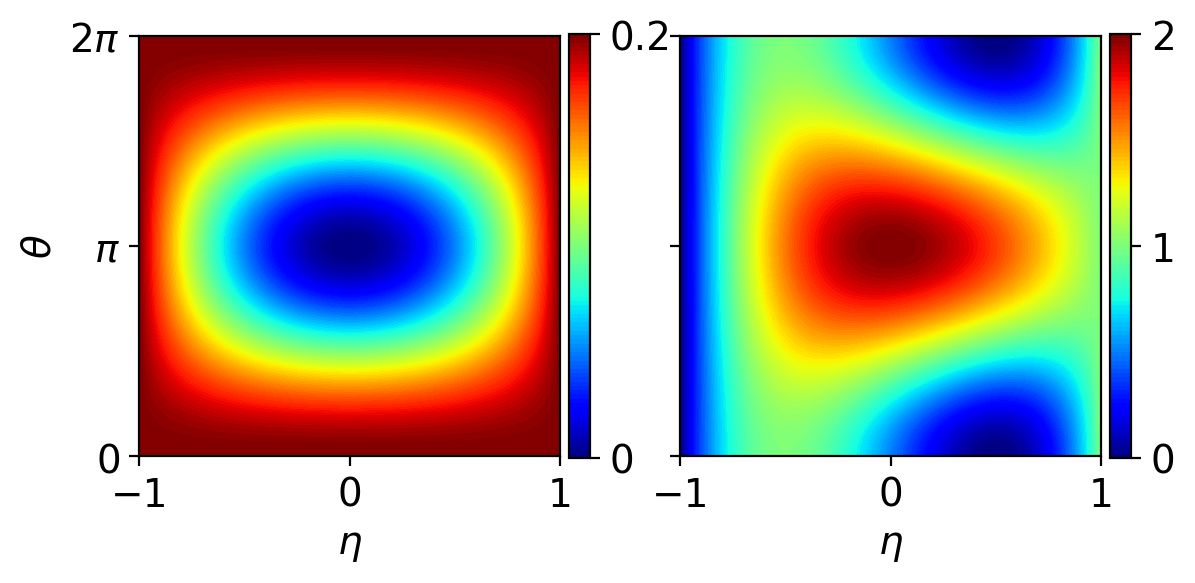
\includegraphics[width=0.8\textwidth]{gfx/ch-spin2/a20-a30-varying.png}
    \caption[Spin-singlet duo and trio amplitudes in a parameter space of
        \(\chi \) and \(\eta \)]
    {\label{fig: UN-BN-duo-trio} Spin singlet-duo (left) and -trio
        (right) amplitudes for the interpolating spinor in
        Eq.~\eqref{eq: UN-BN-interpolating-spinor}.
        Due to the spatially-dependent \(\eta \), this spinor continuously
        interpolates between the UN, BN, and cyclic phases depending on the
        relative phase difference \(\chi=\chi_2+\chi_{-2}-2\chi_0\).}
\end{figure}
Upon investigation, we see interesting behaviour arise in both quantities.
In particular, we see that this spinor can interpolate between the different
phases of UN, BN and cyclic depending on both \(\eta \) and the relative phase
difference \(\chi \).
For example, if one were to maintain \(\theta=0\) and interpolate \(\eta \),
then there would be multiple transitions between the UN (\(|A_{20}|^2 = 1\)) and
BN (\(|A_{20}|^2 = 0\)) phases.
In addition, maintaining a relative phase difference of \(\chi=\pi \), the
singlet-trio amplitude reveals that a cyclic phase is present when
\(-0.5 \lesssim \eta \lesssim 0.5\).
As we shall see in our numerical investigations, this has profound effects on
the structure of topological defects connecting across such an interface.

\subsubsection{Connections involving phase vortices}
To begin our investigations of defects connecting across topological interfaces,
we first consider vortex connections.
We start by constructing a connection of \(k\)-quantised phase vortices on
either side of the interface, which can be achieved by allowing
\(\chi_m=k\varphi\) in Eq.~\eqref{eq: UN-BN-interpolating-spinor}, which results
in a spatially overlapping \(2k\pi \) phase winding in each component.
Such a spinor is given explicitly as
\begin{align}\label{eq: UN-BN-SQV-SQV}
    \zeta_\text{pv-pv}^\text{UN-BN} =
    \frac{1}{2}\mqty(
        e^{ik\varphi}\sqrt{1-\eta} \\
        0 \\
        e^{ik\varphi}\sqrt{2(1+\eta)} \\
        0 \\
        e^{ik\varphi}\sqrt{1-\eta}
    ).
\end{align}
Note that an alternative construction of the above interface is achieved using
Eq~\eqref{eq: general-defect-interface} with\(\tau=k\varphi \) and the Euler
angles kept constant, which then acts on the uniform spinor in
Eq.~\eqref{eq: UN-BN-interpolating-spinor} with \(\chi_m=0\).
One can see that in the above spinor we recover the individual phase vortex
case in both the UN \(\zeta^\text{UN}_\text{pv} = {(0,0,e^{ik\varphi},0,0)}^T\)
and BN \(\zeta^\mathrm{BN}_\text{pv} =
{(e^{ik\varphi},0,0,0,e^{ik\varphi})}^T/\sqrt{2}\) limits when \(\eta = \pm 1\),
respectively.
It is important to note that, despite being characterised by the same phase
winding, the phase vortices on either side of the interface represent entirely
different objects due to the differing topologies of the UN and BN phases.

Instead of connecting two vortices on either side of the interface, one can
instead construct a vortex that terminates on the interface itself, essentially
connecting to a vortex-free region on the other side.
This can be achieved by selectively removing the phase winding from particular
components.
For example, to achieve a \(k\)-quantised phase vortex in the UN limit that
connects to a vortex-free region in the BN limit, we can set \(\chi_0 = 0\) and
\(\chi_{\pm 2} = k\varphi \) in Eq.~\eqref{eq: UN-BN-interpolating-spinor},
which gives
\begin{align}\label{eq: UN-BN-pv-vf}
    \zeta^\text{UN-BN}_\text{pv-vf} = \frac{1}{2}\mqty(
        \sqrt{1-\eta} \\
        0 \\
        e^{ik\varphi} \sqrt{2(1+\eta)} \\
        0 \\
        \sqrt{1-\eta}
    ).
\end{align}
Similarly, by reversing this and setting the winding \(\chi_{\pm 2} = 0\) and
\(\chi_0=k\varphi \) one instead constructs a \(k\)-quantised phase vortex in
the BN phase which connects to a vortex-free region in the UN limit, given by
the spinor
\begin{align}\label{eq: UN-BN-vf-pv}
    \zeta^\text{UN-BN}_\text{vf-pv} = \frac{1}{2}\mqty(
        e^{ik\varphi} \sqrt{1-\eta} \\
        0 \\
        \sqrt{2(1+\eta)} \\
        0 \\
        e^{ik\varphi} \sqrt{1-\eta}
    ).
\end{align}

\subsubsection{Connections involving spin vortices}
Vortices other than singular phase vortices may also be connected across the
interface.
One such example is of singular spin vortices, which, allowing for the fact that
spinor BECs support the non-dissipative flow of spin, carry a circulation only
in the condensate spin and not the mass (see Sec.~\ref{sec: vortices-spin-2}).
An example containing a \(k\)-quantised spin vortex in the BN phase can be
constructed by considering opposite phase windings in the outer components,
i.e., choosing \(\chi_{\pm 2} = \pm \varphi \) in
Eq.~\eqref{eq: UN-BN-interpolating-spinor}, resulting in the spinor
\begin{align}\label{eq: UN-BN-vf-sv}
    \zeta_\text{vf-sv}^\text{UN-BN} = \frac{1}{2}\mqty(
        e^{ik\varphi}\sqrt{1 - \eta} \\
        0 \\
        \sqrt{2(1+\eta)} \\
        0 \\
        e^{-ik\varphi}\sqrt{1 - \eta}
    ).
\end{align}
Since there is no condensate phase winding in the \(\zeta_0\) component in the
above equation, this implies that the spin vortex exists only within the BN
limit, and therefore smoothly connects to a vortex-free state in the UN limit.
It is, however, possible to construct a \(k\)-quantised spin vortex on both
sides of the interface using spin rotations.
Applying the spin rotation \(U(\alpha=k\varphi/2, \beta=\pi/2,\gamma=0)\) to the
initial interpolating spinor in Eq.~\eqref{eq: UN-BN-interpolating-spinor}
results in
\begin{align}\label{eq: UN-BN-sv-sv}
    \zeta_\text{sv-sv}^\text{UN-BN} = \frac{1}{4}\mqty(
        e^{-ik\varphi}(\sqrt{1 - \eta} + \sqrt{3(1+\eta)}) \\
        0 \\
        \sqrt{6(1-\eta)} - \sqrt{2(1+\eta)} \\
        0 \\
        e^{ik\varphi}(\sqrt{1 - \eta} + \sqrt{3(1+\eta)})
    ).
\end{align}
The result of the spin rotation means that in the UN (\(\eta = 1\)) and
BN (\(\eta = -1\)) limits we now have a three-component spinor given,
respectively, as
\begin{align}
    \zeta^\text{UN}_\text{sv} = \mqty(
        e^{-ik\varphi}\sqrt{6} \\ 0 \\ 2 \\ 0 \\ e^{ik\varphi}\sqrt{6}
        ),
    \quad
    \zeta^\text{BN}_\text{sv} = \mqty(
        e^{-ik\varphi}\sqrt{2} \\ 0 \\ 2\sqrt{3} \\ 0 \\ e^{ik\varphi}\sqrt{2}
    ),
\end{align}
thereby allowing spin vortices to appear in both phases, and hence connect
across the topological interface.

\subsubsection{Connections involving half-quantum vortices}
As discussed in Sec.~\ref{sec: vortices-spin-2}, the BN phase supports vortices
which have a fractional winding of the condensate phase, the spin, or a
combination of both.
The charge of such a vortex can be described as (\(w, \sigma\)), where
\(2\pi w\) denotes the winding of the condensate phase, \(\tau\), and
\(2\pi\sigma\) denotes the winding of the spin about some axis of symmetry.
A \((1/2, 1/4)\) HQV in the BN phase can be constructed from
Eq.~\eqref{eq: UN-BN-interpolating-spinor} using the choice \(\chi_2=\chi_0=0\)
and \(\chi_2=\varphi\), which connects it to a vortex-free state in the UN
limit.
Such an interpolating spinor reads
\begin{align}
    \zeta^\text{UN-BN}_\text{vf-hqv} = \frac{1}{2}\mqty(
        \sqrt{1-\eta} \\
        0 \\
        \sqrt{2(1+\eta)} \\
        0 \\
        e^{i\varphi}\sqrt{1-\eta}
    ).
\end{align}
Note that \(\chi_2=\varphi\) and \(\chi_0=\chi_{-2}=0\) would also connect
a HQV in the BN phase to a vortex-free region in the UN phase.
The same \((1/2, 1/4)\) HQV in the BN phase can connect to a singly quantised
phase vortex in the UN limit by allowing \(\chi_2=0\) and
\(\chi_0=\chi_{-2}=\varphi\), resulting in the spinor
\begin{align}
    \zeta^\text{UN-BN}_\text{pv-hqv} = \frac{1}{2}\mqty(
        \sqrt{1-\eta} \\
        0 \\
        e^{i\varphi}\sqrt{2(1+\eta)} \\
        0 \\
        e^{i\varphi}\sqrt{1-\eta}
    ).
\end{align}
A summary of the possible phase, spin, and half-quantum vortex connections
across a UN-BN interface are listed in Table~\ref{tab: UN-BN-vortices}.
\begin{table}
    \centering
    \begin{tabular}{cccccc}
        \toprule
        \multicolumn{5}{c}{UN-BN --- Vortices from spinor-component phase
        winding} \\
        \midrule
        UN limit & BN limit &  \(\chi_2/\varphi \) & \(\chi_0/\varphi \) &
        \(\chi_{-2}/\varphi \)  \\
        \midrule
        Phase vortex & Phase vortex & \(k\) & \(k\) &
         \(k\) \\ 
         Vortex-free & Phase vortex & \(k\) & 0 & \(k\) \\
        Phase vortex & Vortex-free & 0 & \(k\) & 0\\
         Vortex-free & Spin vortex  & \(-k\) & 0 & \(k\) \\
        Phase vortex & Spin vortex  & \(-k\) & \(k\) &
         \(k\) \\
         Vortex-free & Half-quantum vortex  & 0 & 0 & 1 \\
        Phase vortex & Half-quantum vortex  & 0 & \(\pm 1\) & 1 \\
        \bottomrule
    \end{tabular}
    \caption[Examples of possible vortex connections across a uniaxial nematic
    to biaxial nematic interface]{\label{tab: UN-BN-vortices}
    Representative examples of different vortex connections possible across a
    UN-BN interface, constructed from the winding of the phase coefficients
    \(\chi_m\) in Eq.~\eqref{eq: UN-BN-interpolating-spinor}.
    Additionally, generalisations to multiply quantised vortices are given by
    \(k \in \mathbb{Z}\).}
\end{table}

\subsubsection{Connections involving monopoles and nonsingular textures}
So far, we have considered only singular vortices connecting across the
interface.
It is, however, possible to construct interpolating solutions that contain
other types of defects, such as monopoles and nonsingular textures.
For example, the UN phase supports nonsingular spin vortices, which are defined
by a fountain-like texture of the nematic director, \(\hat{\vb{d}} =
(\cos\alpha\sin\beta, \sin\alpha\sin\beta, \cos\beta)\).
The nonsingular fountain-like texture can be achieved by having \(\beta\) be a
monotonically increasing function of the radial coordinate, \(\rho\).
Applying the spin rotation \(U(\alpha=\varphi, \beta=\beta(\rho), \gamma=0)\) to
Eq.~\eqref{eq: UN-BN-interpolating-spinor} with \(\chi_m=0\) results in the
spinor
\begin{align}\label{eq: UN-BN-nsv-sv}
    \zeta^\text{UN-BN}=\frac{1}{\sqrt{2}}\left(
        \sqrt{1+\eta}\zeta^\text{UN}_\text{nsv} + 
        \sqrt{1-\eta}\zeta^\text{BN}_\text{sv}
        \right),
\end{align}
where the UN and BN single phase limits are given, respectively, as
\begin{align}\label{eq: UN-general}
    \zeta^\text{UN}_\text{nsv} &= \sqrt{\frac{3}{8}}
    \mqty(
        e^{-2i\varphi}\sin^2\beta(\rho) \\
        e^{-i\varphi}\sin 2 \beta(\rho) \\
        \frac{1}{\sqrt{6}}\left[1+3\cos 2\beta(\rho)\right] \\
        -e^{i\varphi} \sin 2 \beta(\rho) \\
        e^{2i\varphi}\sin^2\beta(\rho)
    ), \\
    \zeta^\text{BN}_\text{sv} &= \frac{1}{\sqrt{8}} \label{eq: BN-general}
    \mqty(
        e^{-2i\varphi}\left(\cos^2\beta(\rho) + 1\right) \\
        - e^{-i\varphi}\sin 2 \beta(\rho) \\
        \sqrt{6}\sin^2\beta(\rho) \\
        e^{i\varphi}\sin 2 \beta(\rho) \\
        e^{2i\varphi}\left(\cos^2\beta(\rho) + 1\right)          
    ).
\end{align}
This spinor now represents a connection between a nonsingular spin vortex in the
UN limit which smoothly connects to a singular spin vortex in the BN limit.

Since \(\pi_2(\mathcal{M}_\text{UN}) \neq 0\) (see
Sec.~\ref{subsec: spin-2-homotopy}), an interesting example can be
constructed by thinking about a monopole placed in one the UN side of the
interface.
In such an interface, a monopole may form at the termination point of a singular
line vortex.
Similar structures, called boojums, have been observed in
\(^3\)He~\cite{Volovik2009, Blaauwgeers2002}.
A monopole can be realised as a radial hedgehog texture of the nematic director,
\(\vb{\hat{d}}\).
This achieved via the spin rotation \(U(\alpha=\varphi, \beta=\theta,
\gamma=0)\), where \(\theta\) is the polar angle in spherical coordinates.
Applying this spin rotation to the state in
Eq.~\eqref{eq: UN-BN-interpolating-spinor} with \(\chi_m=0\) results in
\begin{align}\label{eq: UN-BN-mp-sv}
    \zeta^\text{UN-BN}=\frac{1}{\sqrt{2}}\left(
        \sqrt{1+\eta}\zeta^\text{UN}_\text{mp} + 
        \sqrt{1-\eta}\zeta^\text{BN}_\text{sv}
        \right),
\end{align}
where the UN and BN single phase limits are given, respectively, as
\begin{align}
    \zeta^\text{UN}_\text{mp} &= \sqrt{\frac{3}{8}}
    \mqty(
        e^{-2i\varphi}\sin^2\theta \\
        e^{-i\varphi}\sin 2 \theta \\
        \frac{1}{\sqrt{6}}\left(1+3\cos 2\theta\right) \\
        -e^{i\varphi} \sin 2 \theta \\
        e^{2i\varphi}\sin^2\theta
    ), \\
    \zeta^\text{BN}_\text{sv} &= \frac{1}{\sqrt{8}}
    \mqty(
        e^{-2i\varphi}\left(\cos^2\theta + 1\right) \\
        - e^{-i\varphi}\sin 2 \theta \\
        \sqrt{6}\sin^2\theta \\
        e^{i\varphi}\sin 2 \theta \\
        e^{2i\varphi}\left(\cos^2\theta + 1\right)          
    ).
\end{align}
This interpolating spinor describes a monopole in the UN limit that terminates
on a singular spin vortex in the BN limit.
A summary of types of defects one can construct using Euler angles in a UN-BN
interface is given in Table~\ref{tab: UN-BN-nonsingular}.
\begin{table}
    \centering
    \begin{tabular}{ccccc}
        \toprule
        \multicolumn{5}{c}{UN-BN --- Vortices, textures, and monopoles using
        Euler angles} \\
        \midrule
        UN limit & BN limit &  \(\alpha/\varphi \) & \(\gamma/\varphi \)
            & \(\beta \) \\
        \midrule
        Spin half-quantum vortex & Spin half-quantum vortex & 1 & 0
            & \(\pi/2\) \\
        Nonsingular spin vortex & Spin vortex & 1 & 0
            & \(\beta\) \\
        Monopole & Spin vortex & 1  & 0 & \(\theta \) \\
        Spin vortex & Monopole & 1 & -1 & \(\beta\) \\ 
        \bottomrule
    \end{tabular}
    \caption[Examples of monopole and nonsingular vortex connections across a
    uniaxial nematic to biaxial nematic interface]
    {\label{tab: UN-BN-nonsingular}
    Summary of other types of defect connections possible in a UN-BN interface.
    Given solutions are characterised by winding of the condensate phase,
    \(\tau \), and Euler angles (\(\alpha, \beta, \gamma \)), expressed in units
    of the azimuthal angle \(\varphi \).
    Here, \(k\) is an integer which provides a generalisation to higher
    quantisation.
    Additionally, \(\theta \) is the polar angle in spherical coordinates, and
    \(\beta\) describes a monotonically increasing function of the
    transverse radius \(\rho \).}
\end{table}

\subsection{Cyclic to nematic}
As we have discussed already in the context of vortex cores, topological
interfaces can arise between the cyclic and nematic phases.
From Fig.~\ref{fig: UN-BN-duo-trio}, we see that by maintaining a constant
\(\chi=\pi \) one can interpolate between the UN, cyclic and BN states.
This can be achieved by the following family of spinors
\begin{align}\label{eq: C-N-interpolating-spinor}
    \zeta^\text{C-N} = \frac{1}{2}\mqty(
    e^{i\chi_2}\sqrt{1 - \eta} \\
    0 \\
    ie^{i\chi_0}\sqrt{2(1+\eta)} \\
    0 \\
    e^{i\chi_{-2}}\sqrt{1 - \eta}
    ),
\end{align}
where we now require that \(\chi_2 + \chi_{-2} - 2\chi_0 = 0\).
Then, due to the \(i\) term in the middle component, this leads to a constant
phase difference of \(\chi_2 + \chi_{-2} - 2(\chi_0 + \pi/2) = -\pi \), and
hence allows us to use the quadratic Zeeman shift to interpolate the above
solution between the different phases.
At \(\eta = 0\) the above solution becomes the three component cyclic state with
a spinor of the form \(\zeta_\mathrm{C} = {(1, 0, i\sqrt{2}, 0, 1)}^T/2\).
The sign of the quadratic Zeeman shift determines which nematic state is chosen,
where \(\eta = \pm 1\) recovers the familiar UN and BN states, respectively.

The uniform mean-field energy of Eq.~\eqref{eq: C-N-interpolating-spinor} reads
\begin{equation}
    E^\text{C-N} = \frac{c_2n}{10}\eta^2 + 2q(1 - \eta).
\end{equation}
The energy becomes minimised at \(\eta = 10q/c_2n\) for \(c_2 > 0\) and fixed
\(q\).
Since the interpolating spinor \(\zeta^\text{C-N}\) is a function of \(q\) only,
the stability of the interface is guaranteed since \(E^\text{C-N} =
2q-10q^2/c_2 \leq E^\text{C}, E^\text{UN},
E^\text{BN}\) for \(|q| < c_2n/10\).
Here, for simplicity, we focus on an interface between the cyclic and BN phases
which is achieved from a longitudinally-dependent quadratic Zeeman shift
\(q(z)\) which varies from \(q = 0\) at the cyclic phase to \(q = -c_2n/10\)
at the BN side.

\subsubsection{Connections involving phase and spin vortices}
Firstly, one can construct the same phase vortex and spin vortex connections
considered in the UN-BN interface upon the substitution \(\sqrt{1+\eta}
\rightarrow i\sqrt{1+\eta}\).
For example, a connection between \(k\)-quantised phase vortices is obtained
from Eq.~\eqref{eq: UN-BN-SQV-SQV}, where the resulting spinor reads
\begin{align}
    \zeta^\text{C-N}_\text{pv-pv} = \frac{1}{2}\mqty(
        e^{ik\varphi}\sqrt{1 - \eta} \\
        0 \\
        ie^{ik\varphi}\sqrt{2(1 + \eta)} \\
        0 \\
        e^{ik\varphi}\sqrt{1 - \eta}
    ),
\end{align}
identifying the cyclic limit as \(\eta = 0\).
This is obtained from Eq.~\eqref{eq: C-N-interpolating-spinor} by the choice
\(\chi_2=\chi_0=\chi_{-2}=k\varphi\).
Additionally, a connection involving spin vortices is constructed as
\begin{align}
    \zeta^\text{C-N}_\text{sv-sv/vf} = \frac{1}{2}\mqty(
        e^{-ik\varphi}\sqrt{1 - \eta} \\
        0 \\
        i\sqrt{2(1 + \eta)} \\
        0 \\
        e^{ik\varphi}\sqrt{1 - \eta}
    ),
\end{align}
which equates to spin vortices in the cyclic and BN limits, connecting to a
vortex-free state in the UN limit.
These connections can be achieved from Eq.~\eqref{eq: C-N-interpolating-spinor}
with the choice \(\chi_{\pm 2} = \mp k\varphi\) and \(\chi_0=0\).
Vortices that can be constructed from component phase windings are summarised in
Table~\ref{tab: C-N-vortices}.
It is worth noting that choosing the phase windings \(\chi_m\) in
Eq.~\eqref{eq: C-N-interpolating-spinor} such that \(\chi \neq 0\) leads
to defect states which are undefined in the cyclic limit, and hence we omit
them from the discussion.
\begin{table}
    \centering
    \begin{tabular}{cccccc}
        \toprule
        \multicolumn{6}{c}{C-N --- Vortices from spinor-component phase
            winding} \\
        \midrule
        Cyclic limit & UN limit & BN limit & \(\chi_2/\varphi \) &
        \(\chi_0/\varphi \) & \(\chi_{-2}/\varphi \) \\
        \midrule
            Phase vortex & Phase vortex & Phase vortex & \(k\) & \(k\) & \(k\)\\
            Spin vortex & Vortex-free & Spin vortex & \(-k\)
            & 0 & \(k\) \\
        \bottomrule
    \end{tabular}
    \caption[Examples of possible vortex connections across a cyclic to nematic
    interface]{\label{tab: C-N-vortices}Summary of the phase and spin vortices
    possible in a cyclic to nematic interface.
    Different vortices are constructed from appropriate choices of the phase
    windings \(\chi_m\).
    Note that \(\chi=0\) for all cases considered as to
    ensure identifiable vortices within the cyclic limit.}
\end{table}

In addition to these connections, it is also possible to construct topologically
distinct spin vortex connection between the cyclic and both nematic phases.
This arises from the common axis of symmetry between the cyclic and BN phases
(see \(C_2'\) axis in Fig.~\ref{fig: nematic-graph}b).
A spin rotation around this particular axis can be achieved by using the
following spin rotation, given here in axis-angle representation:
\begin{align}
    U(C_2', \delta) = \exp\left\{
        -i\frac{\hat{F}_x + \hat{F}_y}{\sqrt{2}}\delta
    \right\},
\end{align}
where \(C_2'\) represents the axis being rotated about and \(\delta\) represents
the angle of rotation.
When \(\delta\) is chosen to be the azimuthal angle such that it winds by
\(2\pi \) about a vortex core (\(\delta=\varphi\)), then the above spin rotation
applied the general cyclic to nematic spinor in
Eq.~\eqref{eq: C-N-interpolating-spinor} results in the following spinor:
\begin{align}
    \zeta^\text{C-N}_\mathrm{sv-sv} = \frac{1}{\sqrt{2}}\left(
    i\sqrt{1+\eta}\zeta^\mathrm{UN}_\mathrm{sv} +
    \sqrt{1-\eta}\zeta^\mathrm{BN}_\mathrm{sv}
    \right), \label{eq: C-BN-sv-sv}
\end{align}
where the spinors in the UN and BN limits are given as
\begin{gather}
    \zeta^\mathrm{UN}_\mathrm{sv} = \sqrt{\frac{3}{8}}
    \mqty(
    \sin^2 \varphi \\
    e^{\frac{i\pi }{4}} \sin 2\varphi \\
    \frac{i}{\sqrt{6}}\left(1 + 3\cos 2\varphi \right)\\
    e^{-\frac{i \pi }{4}} \sin2 \varphi \\
    -\sin^2 \varphi
    ), \\
    \zeta^\mathrm{BN}_\mathrm{sv} = \frac{1}{\sqrt{2}}
    \mqty(
    \cos \varphi \\
    e^{-\frac{3i\pi }{4}} \sin \varphi \\
    0\\
    e^{-\frac{i \pi }{4}} \sin \varphi \\
    \cos \varphi
    ).
\end{gather}
This yields a connection between singular, singly quantised spin vortices in all
three limits.

\subsubsection{Connections involving monopoles and nonsingular textures}
As discussed in the previous section, the nematic phases give rise to
nonsingular spin vortices and point defects such as monopoles.
Those same defect connections can be constructed in this interface by using
the transformation \(\sqrt{1+\eta} \rightarrow i\sqrt{1+\eta}\) in
Eq.~\eqref{eq: UN-BN-nsv-sv} and Eq.~\eqref{eq: UN-BN-nsv-sv}.
This then still results in, for example, the nonsingular vortex/monopole in the
UN limit, which now also connects/terminates to a singular spin vortex in the
cyclic and BN limits.
These defects are summarised in Table~\ref{tab: C-N-other}.
\begin{table}
    \centering
    \begin{tabular}{ccccc}
        \toprule
        \multicolumn{5}{c}{C-N --- Vortices, textures, and monopoles using Euler
            angles} \\
        \midrule
        Cyclic / BN limits & UN limit & \(\alpha/\varphi \)
        & \(\gamma/\varphi \) & \(\beta \) \\
        \midrule
        Spin vortex & Spin vortex & \(\alpha=\pi/4\)
            & \(\gamma=-\alpha\) & \(k\varphi\) \\
        Spin vortex & Nonsingular spin vortex & 1 & 0
            & \(\beta\) \\
        Spin vortex & Monopole & 1 & 0 & \(\theta\) \\
        \bottomrule
    \end{tabular}
    \caption[Examples of monopole and nonsingular vortex connections across a
    cyclic to nematic interface]{\label{tab: C-N-other}Summary of other types of
    defect structures possible in a cyclic to nematic interface.
    Each defect is identified by windings of the condensate phase \(\tau \) and
    Euler angles (\(\alpha, \beta, \gamma \)), expressed in terms of the
    azimuthal angle \(\varphi \).
    For nonsingular vortices, \(\beta\) denotes a monotonically increasing
    function of the transverse radius \(\rho \).
    Additionally, for the monopole case, \(\theta \) is the polar angle in
    spherical coordinates.}
\end{table}

\subsection{Cyclic to ferromagnetic}
Since spin-2 BECs support an FM phase, which has inherent
magnetisation, one can construct an interface between this state and
one with zero magnetisation.
This would then result in spatially distinct regions which have different values
of the spin magnitude, and hence would create a spatially-dependent
magnetisation.
By restricting ourselves to the case of zero transverse magnetisation,
\(\hat{\vb{F}} = \hat{F}_z\), one such case that arises is between the cyclic
and FM phases, given by the following family of spinors:
\begin{align}\label{eq: C-FM-interpolating-spinor}
    \zeta^\text{C-FM} = \frac{1}{\sqrt{3}}\mqty(
        e^{i\chi_2}\sqrt{1 + \eta} \\
        0 \\
        0 \\
        e^{i\chi_{-1}}\sqrt{2 - \eta} \\
        0
    ),
\end{align}
where \(\eta \) now becomes the longitudinal magnetisation, \(\hat{F}_z\).
At zero magnetisation, \(\hat{F}_z = 0\), equivalent to setting \(\eta=0\), this
solution becomes the two-component cyclic state given in
Eq.~\eqref{eq: C-2-spinor} which naturally has no magnetisation.
Then, since this is a spin-2 system, the condensate spin is free to vary between
\(\hat{F}_z = 0\) and \(\hat{F}_z = 2\).
Recall from Chapter~\ref{chap: ground-states} that the spin-2 system supports
two FM ground states, one with \(\spinmag = 1\), which we denote
\(\text{FM}_1^\pm\), and another with \(\spinmag = 2\), which we denote
\(\text{FM}_2^\pm\).
Here, the + (-) represents the FM state with spin pointing up (down).
Therefore, this spinor can interpolate between the cyclic and both FM phases,
depending on the value of the condensate spin, \(\hat{F}_z\).

The uniform mean-field energy of the above spinor reads
\begin{equation}
    E^\text{C-FM} = \frac{c_1 n}{2} \eta^2 - (p-q)\eta + 2q,
\end{equation}
which becomes minimised upon the choice \(\eta = (p-q)/c_1n\) for \(c_1 > 0\)
and fixed \(p, q\).
The interface is expected to be stable within the range
\(-c_1n \leq p \leq 2c_1n\) since \(E^\text{C-FM} \leq
E^\text{C}=0, E^{f_z=1} = c_1n/2 + p\).
Therefore, assuming, e.g., \(q=0\), we can stabilise the interface by an
appropriate choice of a longitudinally-dependent linear Zeeman shift \(p(z)\),
where \(p(z) = 0\) represents the cyclic phase, whilst \(p(z) = -c_1n\) and
\(p(z) = 2c_1n\) represent the \(\text{FM}_1\) and \(\text{FM}_2\) phases,
respectively.

\subsubsection{Connections involving phase, spin, and fractional vortices}
Following the procedure similar to the previous interfaces, we first focus on
constructing phase vortices connecting across this topological interface, which
can be obtained by appropriate winding of \(\chi_2\) and \(\chi_{-1}\).
Again, one can construct \(k\)-quantised phase vortices connecting in all three
limits by crossing \(\chi_2 = \chi_{-1} = k\varphi \), which yields
\begin{align}\label{eq: C-FM-pv-pv}
    \zeta^\text{C-FM}_\text{pv-pv} = \frac{e^{ik\varphi}}{\sqrt{3}}\mqty(
        \sqrt{1 + \eta} \\
        0 \\
        0 \\
        \sqrt{2 - \eta} \\
        0
    ),
\end{align}
In addition to these singly quantised vortices, the cyclic phase supports
vortices with fractional charges, such as one-third and two-third vortices (see
Sec.~\ref{sec: vortices-spin-2}).
One can then construct such a vortex in the cyclic limit by limiting the winding
of the phase to only one component.
Due to the spin-gauge symmetry of the FM phase, this choice of winding would
then lead to either singular phase vortices and vortex-free regions in this
limit.
For example, the following spinor connects a one-third vortex in the cyclic
limit to a singular phase vortex in the \(\text{FM}_2^+\) and a vortex-free
region in the \(\text{FM}_1^-\) limit:
\begin{align}\label{eq: C-FM-third-pv}
    \zeta^\text{C-FM}_{\frac{1}{3}\text{-pv}} = \frac{1}{\sqrt{3}}\mqty(
        e^{i\varphi}\sqrt{1 + \eta} \\
        0 \\
        0 \\
        \sqrt{2 - \eta} \\
        0
    ),
\end{align}
which corresponds to the choice of \(\chi_2 = \varphi \) and \(\chi_{-1} = 0\)
in Eq.~\eqref{eq: C-FM-interpolating-spinor}.
Similarly, a two-third vortex in the cyclic limit can connect to a vortex-free
region in the \(\text{FM}_2^+\) limit or a singular phase vortex in the
\(\text{FM}_1^-\) limit, given by the spinor
\begin{align}\label{eq: C-FM-2third-vf}
    \zeta^\text{C-FM}_{\frac{2}{3}\text{-pv}} = \frac{1}{\sqrt{3}}\mqty(
        e^{i\varphi}\sqrt{1 + \eta} \\
        0 \\
        0 \\
        \sqrt{2 - \eta} \\
        0
    ),
\end{align}
equivalent to setting \(\chi_2 = 0\) and \(\chi_{-1}=\varphi \) in
Eq.~\eqref{eq: C-FM-interpolating-spinor}.
Note that equivalent constructions can be made for the above two spinors using
Eq.~\eqref{eq: general-defect-interface} with \(\tau=-\gamma=\varphi/3\) and
\(\tau=2\gamma=2\varphi/3\), respectively.
A summary of the phase vortex connections possible in this interface are
summarised in Table~\ref{tab: C-FM-vortices}.
\begin{table}
    \centering
    \begin{tabular}{ccccc}
        \toprule
        \multicolumn{5}{c}{C-FM --- Vortices from spinor-component phase
            winding} \\
        \midrule
        Cyclic limit & \(\text{FM}_2\) limit & \(\text{FM}_1\) limit
            & \(\chi_2/\varphi \) & \(\chi_{-1}/\varphi \) \\
        \midrule
         Phase vortex & Phase vortex & Phase vortex & \(k\) & \(k\) \\ 
         One-third vortex & Phase vortex & Vortex-free & 1 & 0 \\
         Two-third vortex & Vortex-free & Phase vortex & 0 & 1 \\
         Spin vortex & Phase vortex & Phase vortex & \(-2k\) & \(k\) \\
        \bottomrule
    \end{tabular}
    \caption[Examples of possible vortex connections across a cyclic to
    ferromagnetic interface]{\label{tab: C-FM-vortices}Summary of the vortex
    connections possible in a cyclic to FM interface.
    Each vortex can be constructed by choosing the appropriate phase winding
    \(\chi_m\), expressed in terms of the azimuthal angle \(\varphi \).
    Here, \(k \) is an integer that allows one to represent vortices of
    arbitrary quantisation.}
\end{table}

\subsubsection{Connections involving monopoles and nonsingular textures}
In addition to phase vortices, the FM phase also supports nonsingular vortices,
which are identified from a characteristic fountain-like texture of
the condensate spin (see Fig.~\ref{fig: spin-1-vortices}b for the spin-1
analogue.)
To construct such a defect across an interface, we first construct the most
general C-FM interface spinor by applying the general spin rotation
\(U(\alpha, \beta, \gamma)\) to the interpolating spinor in
Eq.~\eqref{eq: C-FM-interpolating-spinor}, which results in
\begin{align}\label{eq: C-FM-coreless-general}
    \zeta^\text{C-FM} = \frac{1}{\sqrt{3}}\left(
        \sqrt{1 + \eta}\zeta^{\text{FM}_2^+}
        + \sqrt{2 - \eta}\zeta^{\text{FM}_1^-}
    \right),
\end{align}
where the individual FM limits are given as
\begin{align}\label{eq: FM-2-coreless}
    \zeta^{\text{FM}_2^+} =e^{i(\tau-2\gamma)}
    \mqty(
    e^{-2i\alpha}\cos^4\frac{\beta}{2} \\
    2e^{-i\alpha}\cos^3\frac{\beta}{2}\sin\frac{\beta}{2}  \\
    \sqrt{6}\cos^2\frac{\beta}{2}\sin^2\frac{\beta}{2} \\
    2e^{i\alpha}\cos\frac{\beta}{2}\sin^3\frac{\beta}{2} \\
    e^{2i\alpha}\sin^4\frac{\beta}{2}
    ),
\end{align}
\begin{align}\label{eq: FM-1-coreless}
    \zeta^{\text{FM}_1^-} = e^{i(\tau + \gamma)}
    \mqty(
    -2e^{-2i\alpha}\cos\frac{\beta}{2}\sin^3\frac{\beta}{2} \\
    e^{-i\alpha}\sin^2\frac{\beta}{2}\left(
        3\cos^2\frac{\beta}{2} -\sin^2\frac{\beta}{2}
    \right) \\
    \sqrt{6}\left(
        \cos\frac{\beta}{2}\sin^3\frac{\beta}{2}
        - \cos^3\frac{\beta}{2}\sin\frac{\beta}{2}
    \right) \\
    e^{i\alpha}\cos^2\frac{\beta}{2}\left(
        \cos^2\frac{\beta}{2}-3\sin^2\frac{\beta}{2}
    \right) \\
    2e^{2i\alpha}\cos^3\frac{\beta}{2}\sin\frac{\beta}{2}
    ).
\end{align}
To construct the characteristic fountain-like spin texture, we choose \(\beta\)
as a monotonically increasing function of the transverse radius, \(\rho\).
In the \(\text{FM}_2\) and \(\text{FM}_1\) cases, the order-parameter is kept
single-valued by a combined winding of the condensate phase coupled to a winding
of the spin vector, achieved, respectively, by
\begin{align}\label{eq: coreless-euler-limits-FM-2}
    \tau - 2\gamma &= \pm 2\alpha = \pm 2\varphi, \\
    \tau + \gamma &= \pm\alpha=\pm\varphi.\label{eq: coreless-euler-limits-FM-1}
\end{align}
Choosing these Euler angles results in nonsingular vortices in the FM limits
connecting to singular vortices in the cyclic limit.
The type of singular vortex present in the cyclic limit depends on how
\(\gamma\) and \(\tau\) are specifically chosen.
Choosing \(\gamma = 0 \) or \(\tau = 0\) results in phase vortices or spin
vortices, respectively.
Additionally, the choice of \(\tau=\varphi/3\) or \(\tau=2\varphi/3\) results
in fractionally quantised vortices in the cyclic limit connecting to nonsingular
vortices in the FM phases.
The spherical harmonic representation of the nonsingular vortices arising in the
FM phases are shown in Fig.~\ref{fig: C-FM-coreless-initial-states}, where we
see the characteristic fountain-like texture emerge.
\begin{figure}
    \centering
    \begin{tikzpicture}
        \node at (0, 0) {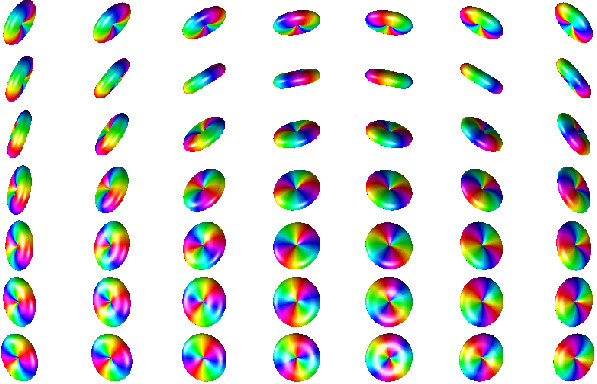
\includegraphics[width=0.45\textwidth]
            {gfx/ch-spin2/FM-2-coreless.pdf}};
        \node at (7.5, 0) {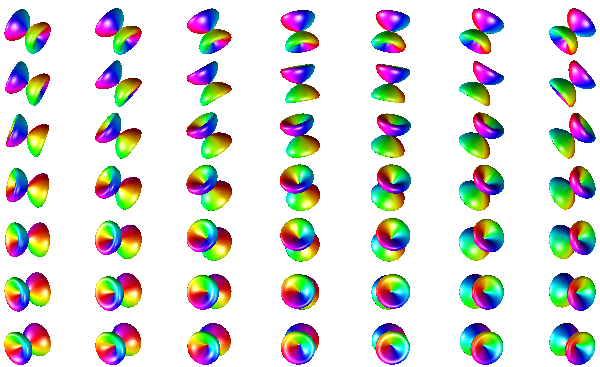
\includegraphics[width=0.47\textwidth]
            {gfx/ch-spin2/FM-1-coreless.pdf}};

        % Colour bar
        \node at (3.25, 2.7){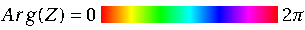
\includegraphics{gfx/colourbars/compiled_hsv.pdf}};

        % Labels
        \node at (0, -2.7) {(a)};
        \node at (7.5, -2.7) {(b)};
    \end{tikzpicture}
    \caption[Spherical harmonic representation of the nonsingular vortices
    arising in a cyclic to ferromagnetic interface.]
    {\label{fig: C-FM-coreless-initial-states}Spherical harmonic
    representation of the nonsingular vortices constructed in
    Eq.~\eqref{eq: C-FM-coreless-general}.
    (a) Nonsingular vortex in the \(\text{FM}_2^+\) limit given by
    Eq.~\eqref{eq: FM-2-coreless} with the choice \(\tau - 2\gamma = 2\alpha
    = 2\varphi \).
    (b) Nonsingular vortex in the \(\text{FM}_1^-\) limit given by
    Eq.~\eqref{eq: FM-1-coreless} with the choice \(\tau + \gamma = \alpha
    = \varphi \).}
\end{figure}

A generalisation of the Dirac monopole, which consists of a hedgehog texture of
the condensate spin, \(\langle \hat{\vb{F}} \rangle\), that terminates on a
singular vortex, can be constructed in the FM phases.
Similar generalisations have already been constructed in spin-1
systems~\cite{Borgh2012, Savage2003}.
Such a structure is achieved by taking \(\beta=\theta\) in
Eqs.~\eqref{eq: FM-2-coreless} and~\eqref{eq: FM-1-coreless}, where \(\theta\)
is the polar angle in spherical coordinates, along with the same required limits
on the Euler angles given in Eqs.~\eqref{eq: coreless-euler-limits-FM-2}
and~\eqref{eq: coreless-euler-limits-FM-1}.
This creates the required hedgehog texture of the condensate spin and embeds
a singular vortex line terminating on the monopole.
These choices of angles then connect the generalisation of the Dirac monopole
in the FM limits to either phase, spin, or fractional vortices in the cyclic
limit using the choice of angles discussed for the nonsingular case.
A table of vortices, textures, and monopoles that can be constructed using
Euler angles in the C-FM interface are presented in Table~\ref{tab: C-FM-other}.
\begin{table}
    \centering
    \begin{tabular}{cccccc}
        \toprule
        \multicolumn{6}{c}{C-FM --- Vortices, textures and monopoles using Euler
            angles} \\
        \midrule
        C limit & \(\text{FM}_2\) limit &  \(\tau/\varphi\) & \(\alpha/\varphi\)
            & \(\gamma/\varphi\) & \(\beta\) \\
        \midrule
        Phase vortex & Nonsingular vortex & 2 & 1 & 0 & \(\beta(\rho)\) \\ 
        Spin vortex & Nonsingular vortex & 0 & 1 & \(\pm 1\)
            & \(\beta(\rho)\) \\ 
        Two-third vortex & Nonsingular vortex & 2/3 & 1 & -2/3, 4/3
            & \(\beta(\rho)\) \\
        Phase vortex & Dirac monopole & 2 & \(1\) & 0 & \(\theta\) \\ 
        Spin vortex & Dirac monopole & 0 & \( 1\) & \(\pm 1\)
            & \(\theta\) \\ 
        Two-third vortex & Dirac monopole & 2/3 & \( 1\) & -2/3, 4/3
            & \(\theta\) \\
        \bottomrule
        \midrule
        C limit & \(\text{FM}_1\) limit &  \(\tau/\varphi\) & \(\alpha/\varphi\)
            & \(\gamma/\varphi\) & \(\beta\) \\
        \midrule
        Phase vortex & Nonsingular vortex & 1 & 1 & 0 & \(\beta(\rho)\) \\ 
        Spin vortex & Nonsingular vortex & 0 & 1 & \(\pm 1\)
            & \(\beta(\rho)\) \\ 
        One-third vortex & Nonsingular vortex & 1/3 & 1 & -4/3, 2/3
            & \(\beta(\rho)\) \\
        Phase vortex & Dirac monopole & 1 & 1 & 0 & \(\theta\) \\ 
        Spin vortex & Dirac monopole & 0 & 1 & \(\pm 1\) & \(\theta\)\\ 
        One-third vortex & Dirac monopole & 1/3 & 1 & -4/3, 2/3 & \(\theta\) \\
        \bottomrule
    \end{tabular}
    \caption[Examples of monopoles and nonsingular vortex connections across a
    cyclic to ferromagnetic interface.]
    {\label{tab: C-FM-other}List of vortices, textures, and monopoles
    that can be constructed in a cyclic to FM interface using a combination
    of the condensate phase \(\tau\) and the Euler angles \(\alpha, \beta,
    \gamma\).
    Here, \(\tau, \alpha, \gamma\) are given as multiples of the azimuthal angle
    \(\varphi\), whilst \(\beta\) is either a multiple of the polar angle
    \(\theta\), or a monotonically increasing function of the transverse radius,
    \(\rho\).}
\end{table}

\subsection{Ferromagnetic to biaxial nematic}
Another interface containing non-zero magnetisation is that between the FM and
BN phases, given by the following family of spinors:
\begin{align}\label{eq: FM-BN-interpolating-spinor}
    \zeta^\text{FM-BN} = \frac{1}{\sqrt{2}}\mqty(
    e^{i\chi_2} \sqrt{1 + \eta} \\
    0 \\
    0 \\
    0 \\
    e^{i\chi_{-2}} \sqrt{1 - \eta}),
\end{align}
where \(\eta \) relates to the longitudinal magnetisation as \(\eta =
\hat{F}_z / 2\).
This state then interpolates between the BN state at \(\eta = 0\), to an FM
state with spin pointing up (down) for \(\eta = 1 (-1)\).
The energy of this interpolating spinor is obtained by substituting the above
into Eq.~\eqref{eq: energy-per-particle}, which reads
\begin{align}\label{eq: FM-BN-energy}
    E^\text{FM-BN} = \frac{n}{2}\left(c_1-\frac{c_2}{20}\right)\eta^2
    - p \eta + 4q + \frac{nc_2}{10}.
\end{align}
This energy becomes minimised precisely when \(\eta = p / [(c_1-c_2/20)n]\) for
\(c_1 \geq c_2/20\) and fixed \(p\) and \(q\).
Substitution of \(\eta = p / [(c_1-c_2/20)n]\) into Eq.~\eqref{eq: FM-BN-energy}
reveals that \(E^\text{FM-BN} \leq E^\text{BN},
E^{\text{FM}_2}\) for \(|p| < (2c_1-c_2/10)n\).
Thus, as in the previous FM interface, we can stabilise the interface by relying
on a longitudinal dependence of the linear Zeeman shift, \(p(z)\).
One can see that at \(p = \pm 2(c_1-c_2/20)n\) the above solution becomes
the FM state with spin \(\eta = \pm 2\).
Alternatively, the solution becomes the BN state precisely when \(p=0\), and
hence has zero magnetisation.
Therefore, this spinor provides an interpolating solution between the
FM and BN phases, which is controlled by a longitudinal dependence of
the linear Zeeman shift, \(p(z)\).

\subsubsection{Connections involving phase, spin, and half-quantum vortices}
We start from the interpolating spinor between the FM and BN phases in
Eq.~\eqref{eq: FM-BN-interpolating-spinor} and first construct various vortex
states using different combinations of the phase windings \(\chi_{\pm 2}\).
Again, similar to the previous cases, \(k\)-quantised phase vortices are
connected across the interface by the choice \(\chi_{\pm 2} = k\varphi \).
An interesting case arises between a \(k\)-quantised phase vortex in the FM
phases connecting to a spin vortex in the BN phase.
This can be achieved by again allowing opposite phase windings in the outer
components, i.e., \(\chi_{\pm 2} = \pm k\varphi \), where the interpolating
spinor reads
\begin{align}\label{eq: FM-BN-pv-sv}
    \zeta^\text{FM-BN}_\text{pv-sv} = \frac{1}{\sqrt{2}}\mqty(
    e^{ik\varphi} \sqrt{1 + \eta} \\
    0 \\
    0 \\
    0 \\
    e^{-ik\varphi} \sqrt{1 - \eta}).
\end{align}

As observed in Fig.~\ref{fig: SV-HQV}, the BN phase allows for the creation
of a HQV, characterised by a half-winding of the condensate phase.
Such a vortex can be constructed by allowing a phase winding in only one of the
outer components, i.e., \(\chi_2 = \varphi \) and \(\chi_{-2} = 0\) or vice
versa.
Using this first choice in Eq.~\eqref{eq: FM-BN-interpolating-spinor} leads to
the spinor
\begin{align}\label{eq: FM-BN-pv-hqv}
    \zeta^\text{FM-BN}_\text{pv-hqv} = \frac{1}{\sqrt{2}}\mqty(
    e^{i\varphi} \sqrt{1 + \eta} \\
    0 \\
    0 \\
    0 \\
    \sqrt{1 - \eta}),
\end{align}
which connects a HQV in the BN limit to a phase vortex in the \(\text{FM}_2\)
limit when \(\eta = 1\), or a vortex-free state when \(\eta = -1\).
Choosing \(\chi_{\pm 2}\) the opposite way around would reverse this connection.
A summary of possible vortex connections constructed using the component phase
windings is provided in Table~\ref{tab: FM-BN-vortices}.
\begin{table}
    \centering
    \begin{tabular}{ccccc}
        \toprule
        \multicolumn{5}{c}{Ferromagnetic to biaxial nematic --- Vortices} \\
        \midrule
        \(\text{FM}_2^+\) limit & \(\text{FM}_2^-\) limit & BN limit
            & \(\chi_2/\varphi \) & \(\chi_{-2}/\varphi \)  \\
        \midrule
         Phase vortex & Phase vortex & Phase vortex & \(k\) & \(k\) \\ 
         Phase vortex & Vortex-free & Half-quantum vortex & 1 & 0 \\
         Vortex-free & Phase vortex & Half-quantum vortex & 0 & 1 \\
         Phase vortex & Phase vortex & Spin vortex  & \(-k\) & \(k\) \\
        \bottomrule
    \end{tabular}
    \caption[Examples of possible vortex connections across a ferromagnetic
    to biaxial nematic interface]{\label{tab: FM-BN-vortices}
    Summary of possible vortex connections across an FM to BN interface.
    Each vortex is given in terms of the winding \(\chi_m\), given in multiples
    of the azimuthal angle \(\varphi \).
    The FM limits are specified by the direction of the condensate spin, where
    a spin pointing up denotes a spinor of the form
    \(\zeta={(1, 0, 0, 0, 0)}^T\), and a spin pointing down denotes a spinor of
    the form \(\zeta={(0, 0, 0, 0, 1)}^T\).
    Additionally, \(k\) is an integer that allows one to generalise to higher
    quantisation.}
\end{table}

\subsubsection{Connections involving monopoles and nonsingular textures}
As in the previous subsection discussing a cyclic to FM interface, we can apply
the same logic and construct nonsingular defects in the FM phase that connect to
singular defects in the BN phase, as well as Dirac monopoles that form the
termination point of vortices.
We begin by re-writing Eq.~\eqref{eq: FM-BN-interpolating-spinor} in the general
form
\begin{align}
    \zeta^\text{FM-BN} = \frac{1}{\sqrt{2}}\mqty(
        \sqrt{1+\eta}\zeta^{\text{FM}_2^+} \\
        0 \\
        0 \\
        0 \\
        \sqrt{1+\eta}\zeta^{\text{FM}_2^-}
    ),
\end{align}
where \(\text{FM}_2^+\) is defined in Eq.~\eqref{eq: FM-2-coreless} and
\(\text{FM}_2^-\) is similarly obtained by applying a general spin rotation
to \(\zeta={(0, 0, 0, 0, 1)}^T\).
Then, choosing the Euler angles according to
Eq.~\eqref{eq: coreless-euler-limits-FM-2} results in \(\text{FM}_2^\pm\)
becoming
\begin{align}
    \zeta^{\text{FM}_2^+} &=
    \mqty(
        e^{-4i\varphi} \cos^4 \frac{\beta}{2} \\
        2e^{-3i\varphi} \cos^3 \frac{\beta}{2} \sin \frac{\beta}{2} \\
        \sqrt{6}e^{-2i\varphi}\cos^2\frac{\beta}{2}\sin^2\frac{\beta}{2}\\
        2e^{-i\varphi} \sin^3 \frac{\beta}{2} \cos \frac{\beta}{2} \\
        \sin^4\frac{\beta}{2}
        \label{eq: FM-BN-dirac2}
    ), \\
    \zeta^{\text{FM}_{2}^-} &= 
    \mqty(
        e^{-4i\varphi} \sin^4 \frac{\beta}{2} \\
        -2e^{-3i\varphi} \sin^3 \frac{\beta}{2} \cos \frac{\beta}{2} \\
        \sqrt{6}e^{-2i\varphi}\cos^2\frac{\beta}{2}\sin^2\frac{\beta}{2}\\
        -2e^{-i\varphi} \cos^3 \frac{\beta}{2} \sin \frac{\beta}{2} \\
        \cos^4\frac{\beta}{2}
    ),
\end{align}
respectively.
Then, choosing \(\beta\) as a monotonically increasing function of the
transverse radius results in nonsingular vortices in both FM limits which
connect to either phase, spin, or HQVs in the BN limit (\(\eta=0\)) depending
on whether \(\tau=2\varphi, 0, \varphi/2\), respectively.
Similarly, choosing \(\beta=\theta\) represents a generalisation of the Dirac
monopole in both FM limits, which connects to either phase, spin, or HQVs in
the BN limit depending on the choice of \(\tau\).
A summary of vortices, textures, and monopoles that can be constructed using
the Euler angles in an FM-BN interface is given in Table~\ref{tab: FM-BN-other}.
\begin{table}
    \centering
    \begin{tabular}{cccccc}
        \toprule
        \multicolumn{6}{c}{FM-BN --- Vortices, textures and monopoles from Euler
            angles} \\
        \midrule
        \(\text{FM}_2\) limit & BN limit & \(\tau/\varphi\) & \(\alpha/\varphi\)
            & \(\gamma/\varphi\) & \(\beta\) \\
        \midrule
        Nonsingular vortex & Phase vortex & \(2\) & 1 & \(0\)
            & \(\beta(\rho)\) \\ 
        Nonsingular vortex & Spin vortex  & \(0\) & 1 & \(\pm 1\)
            & \(\beta(\rho)\) \\ 
        Nonsingular vortex & Half-quantum vortex & 1/2 & 1 & -3/4
            & \(\beta(\rho)\) \\ 
        Dirac monopole & Phase vortex & 2 & 1  & 0 & \(\theta\)\\
        Dirac monopole & Spin vortex & 0 & 1  & \(\pm 1\)
            & \(\theta\)\\
        Dirac monopole & Half-quantum vortex & 1/2 & 1  & -3/4 & \(\theta\) \\
        \bottomrule
    \end{tabular}
    \caption[Examples of monopoles and nonsingular vortex connections across a
    ferromagnetic to biaxial nematic interface.]
    {\label{tab: FM-BN-other}List of vortices, textures, and monopoles
    that can be constructed in an FM to BN interface using a combination
    of the condensate phase \(\tau\) and the Euler angles \(\alpha, \beta,
    \gamma\).
    Here, \(\tau, \alpha, \gamma\) are given as multiples of the azimuthal angle
    \(\varphi\), whilst \(\beta\) is either a multiple of the polar angle
    \(\theta\), or a monotonically increasing function of the transverse radius,
    \(\rho\).}
\end{table}

\section{Numerical investigations of defect crossing physics}
In this section we numerically investigate some topological interfaces defined
in the preceding section, along with a subset of the possible defect
connections.
Our numerical setup is as follows.
We numerically evolve the spin-2 GPEs defined in
Eqs.~\eqref{eq: spin-2-GPEs-pm2} -~\eqref{eq: spin-2-GPEs-0} using a symplectic
integrator~\cite{Symes2017} using, for simplicity, a purely isotropic trapping
potential \(V=M\omega^2r^2/2\).
We simulate the energy loss during experiments by introducing a phenomenological
damping coefficient, \(\nu \), through the substitution
\(t \rightarrow (1-i\nu)t\).
In all simulations considered, we choose \(\nu = 1e-2\).
We perform our simulations on a 3D of \(N_s^3=128^3\) points, with side lengths
\(L = 20\ell \), where \({(\ell =\hbar/M\omega)}^{1/2}\) is the (isotropic)
harmonic oscillator length.
We choose parameters that correspond to a \(^{87}\)Rb
condensate~\cite{Klausen2001} with \(c_0n=1.32\times10^4\hbar\omega\ell^3\),
\(c_0/c_1=90.7\), and \(c_0/c_2=-102\), where the ground state is predicted to
be nematic (see Sec.~\ref{subsec: spin-2-experimental-parameters} for details
on the choice of numerical parameters).
In each simulation, we perform a small spin rotation to the initial state to
avoid components that are identically zero.
Additionally, when constructing states with defects, the position of each defect
is perturbed slightly to avoid artificial stability when placed at exactly the
centre of the trap.
Details of the trapped, dimensionless units can be found in
Sec.~\ref{subsec: spin-2-dimensionless}.

\subsection{\label{subsec: UN-BN-numerics}
Uniaxial nematic to biaxial nematic interface}
The first interface we consider is that between the UN and BN phases, considered
in Sec.~\ref{subsec: UN-BN-defects}.
Since the UN and BN phases are energetically degenerate in the absence of a
magnetic field, we introduce a spatially-dependent quadratic Zeeman shift
\(q(z)\) such that \(q(z) > 0\) on the UN side and \(q(z) < 0\) on the BN side
to lift the degeneracy, and the maximum strength of our quadratic Zeeman shift
is set to \(q_\text{max} = 0.1\hbar\omega \).
The quadratic Zeeman shift linearly interpolates over a small transition region
(which we take to be small compared to the spin-dependent healing lengths) from
\(q = -0.1\hbar\omega \) in the BN phase to \(q = 0.1\hbar\omega \) in the UN
phase.

Our investigation begins with that of the phase vortex connection, where the
initial state is constructed as in Eq.~\eqref{eq: UN-BN-SQV-SQV}.
To imprint the vortices, we perform a short imaginary time propagation, then
proceed to numerically evolve the spin-2 GPEs.
The dynamics of this connection is split into two distinct parts, which are
plotted in Fig.~\ref{fig: UN-BN-SQV-SQV-singlets}.
Firstly, upon evolution, the two overlapping SQVs spatially separate due to an
instability occurring at the interface \(z \approx 0\).
Each phase vortex then connects to a vortex-free state on the other side of the
interface shown in Fig.~\ref{fig: UN-BN-SQV-SQV-singlets}a.
After the initial separation, the cores of the vortices fill with atoms
occupying different ground states, drastically altering the order parameter
symmetry within the cores.
\begin{figure}
    \centering
    \begin{tikzpicture}
        \node at (0, 0) {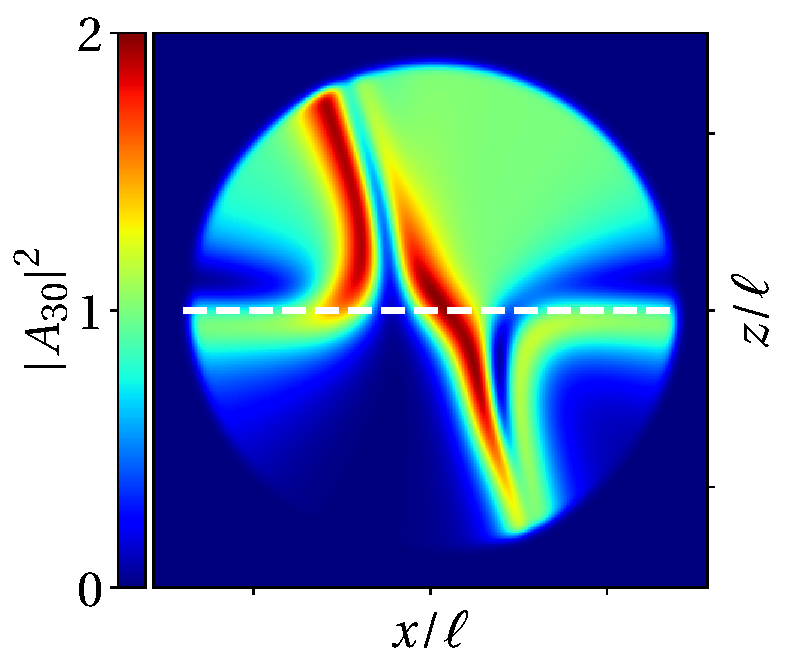
\includegraphics[width=0.33\textwidth]
            {gfx/ch-spin2/UN-BN_SQV-SQV_longitudinal_a30.pdf}};

        \node at (4.8, 2.2) {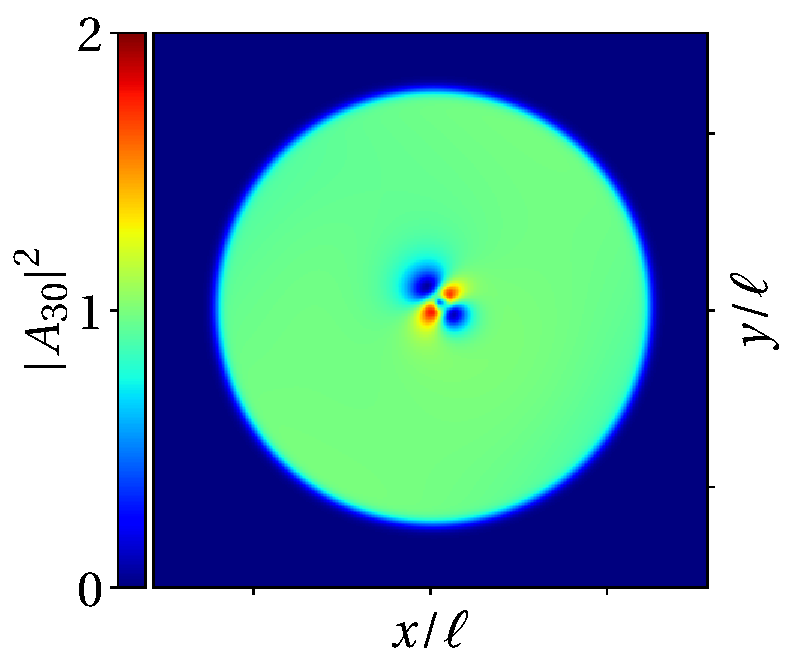
\includegraphics[width=0.33\textwidth]
            {gfx/ch-spin2/UN-BN_SQV-SQV_a30_UN.pdf}};

        \node at (4.8, -2.7) {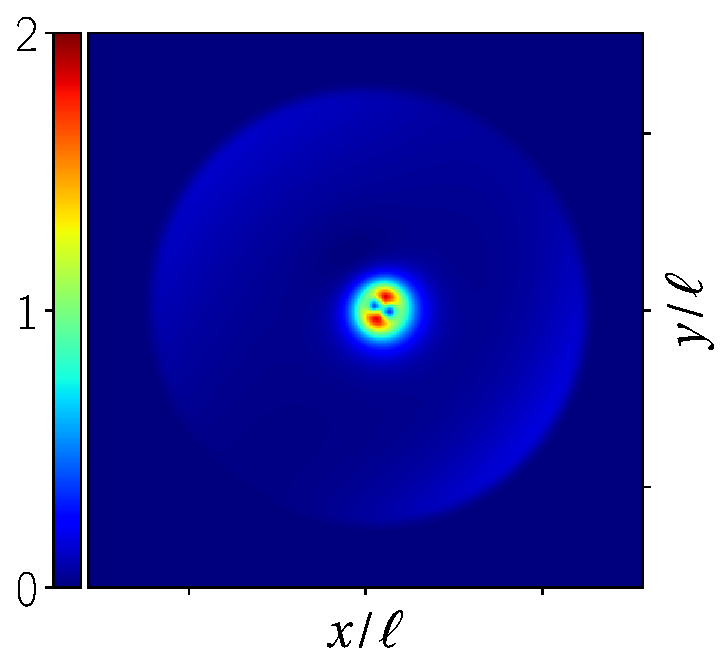
\includegraphics[width=0.33\textwidth]
            {gfx/ch-spin2/UN-BN_SQV-SQV_a30_BN.pdf}};

        \node at (10, 2.35) {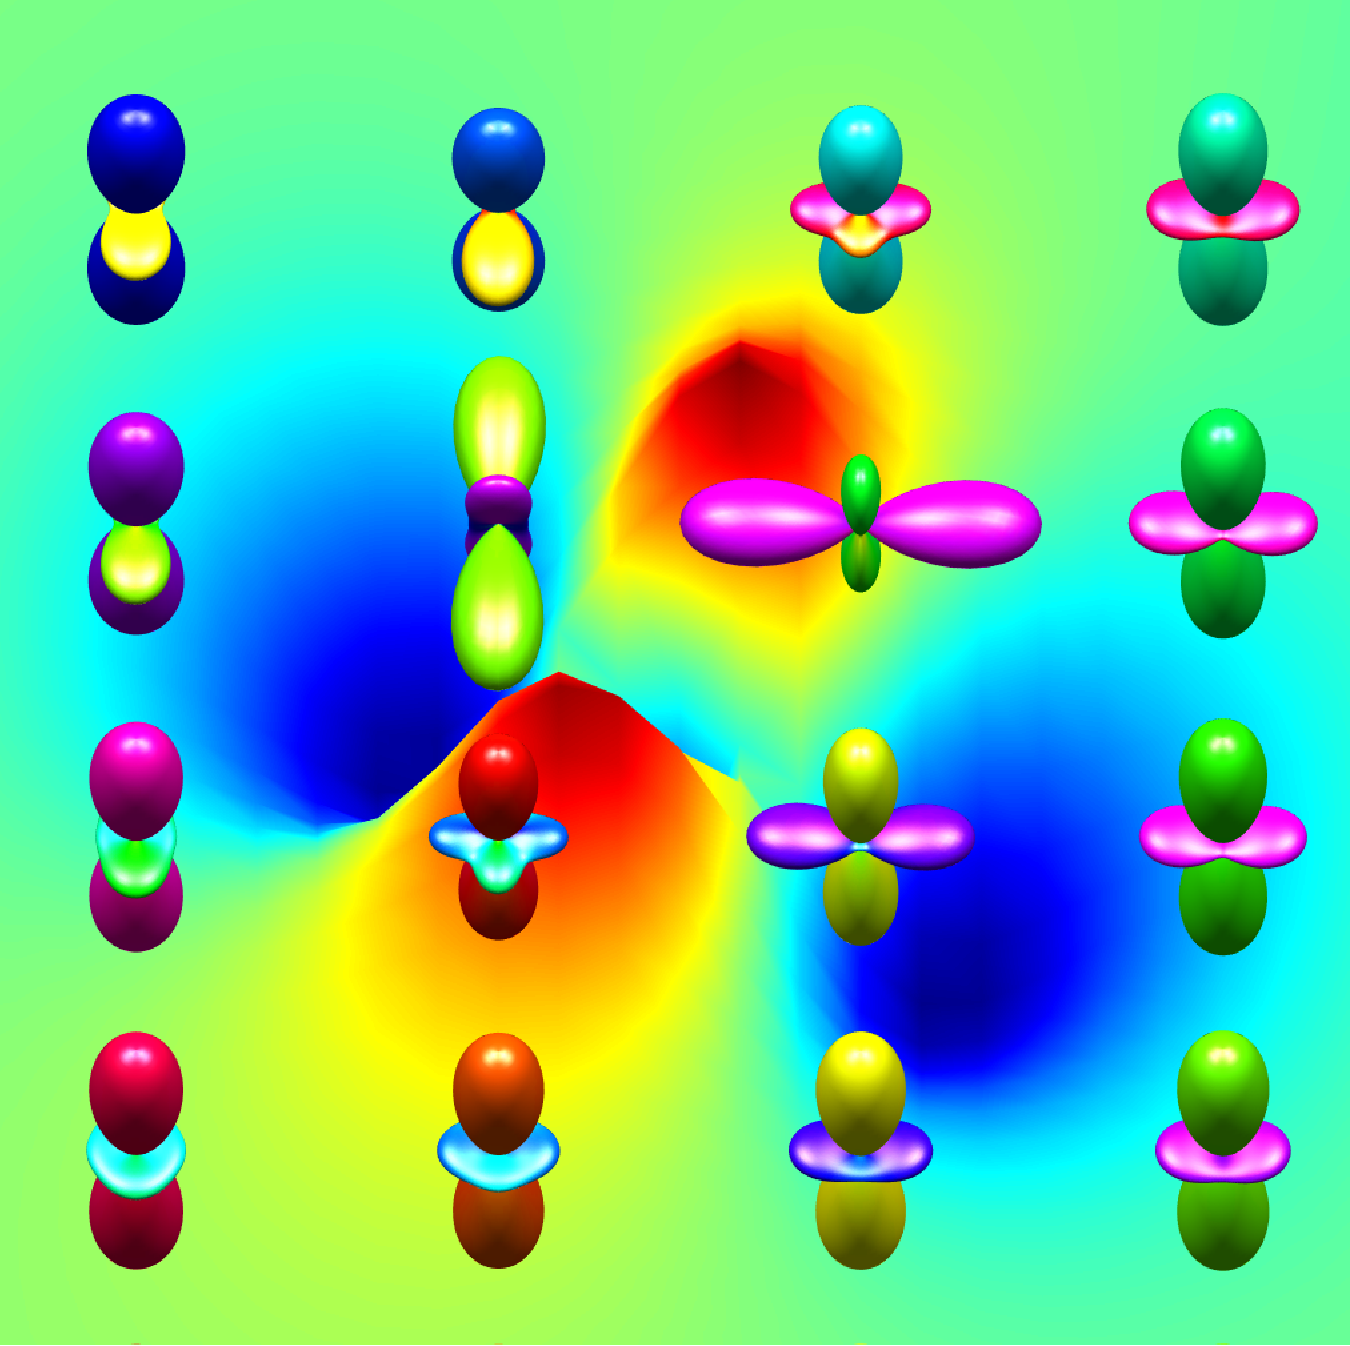
\includegraphics[width=0.26\textwidth]
            {gfx/ch-spin2/UN-BN_SQV-SQV_singletTrio_UN.png}};
        \node[rectangle, draw=black, minimum width=0.55cm,
            minimum height=0.55cm]
        (UN_small_rec) at (5.05, 2.45) {};
        \node[rectangle, draw=black, minimum width=3.8cm,
            minimum height=3.8cm]
        (UN_big_rec) at (10, 2.33) {};
        \draw[-, dashed] (UN_big_rec.north west) -- (UN_small_rec.north west){};
        \draw[-, dashed] (UN_big_rec.south west) -- (UN_small_rec.south west){};

        \node at (10, -2.58) {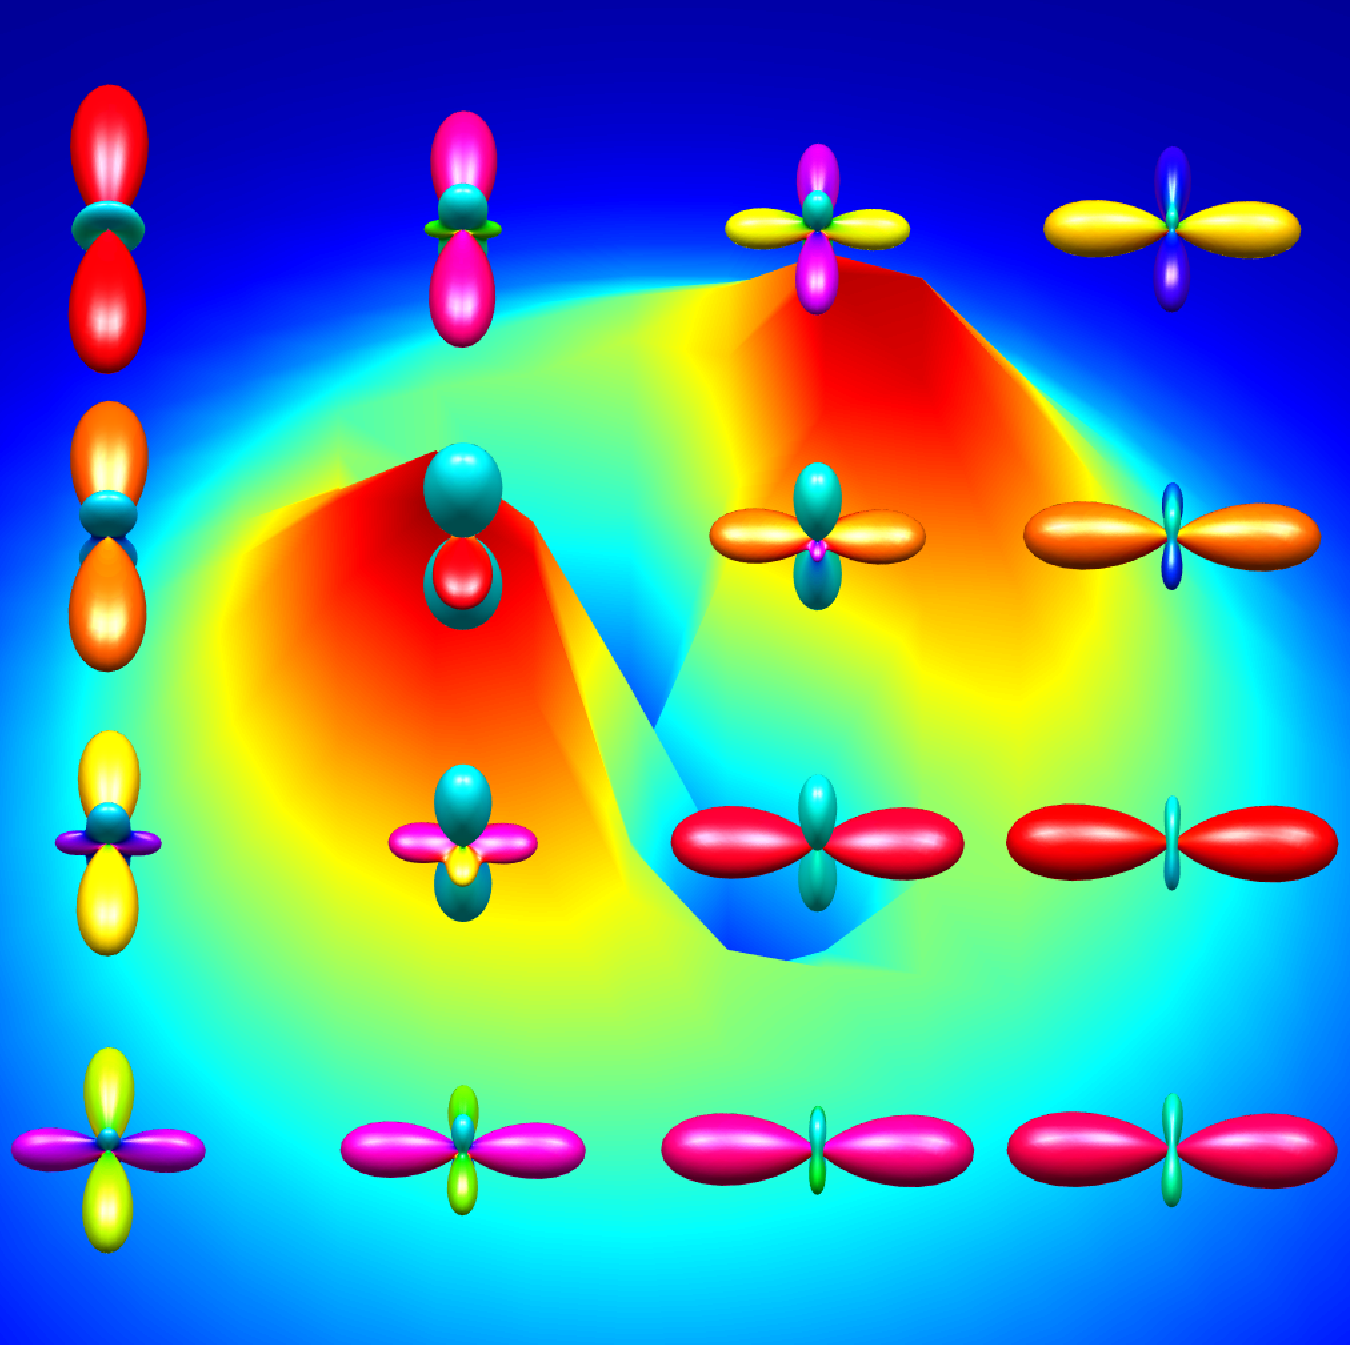
\includegraphics[width=0.26\textwidth]
            {gfx/ch-spin2/UN-BN_SQV-SQV_singletTrio_BN.png}};
        \node[rectangle, draw=black, minimum width=0.55cm,
            minimum height=0.55cm]
        (BN_small_rec) at (5.1, -2.52) {};
        \node[rectangle, draw=black, minimum width=3.8cm,
            minimum height=3.8cm]
        (BN_big_rec) at (10, -2.57) {};
        \draw[-, dashed] (BN_big_rec.north west) -- (BN_small_rec.north west){};
        \draw[-, dashed] (BN_big_rec.south west) -- (BN_small_rec.south west){};

        \node at (0, -2.5) {(a)};
        \node at (5, -0.3) {(b)};
        \node at (5, -5.2) {(c)};
        \node at (10, -0.3) {(d)};
        \node at (10, -5.2) {(e)};
    \end{tikzpicture}
    \caption[Dynamics of a singly quantised vortex connection across a uniaxial
        nematic to biaxial nematic interface]
    {\label{fig: UN-BN-SQV-SQV-singlets}Spin singlet-trio amplitude for
        the UN-BN phase vortex connection given in Eq.~\eqref{eq: UN-BN-SQV-SQV}
        at \(\tilde{t} = 300\).
        (a): Longitudinal cut showing the spatial separation of the two vortex
        lines.
        (b) and (c): Transverse cut on the UN (\(z/\ell = 3.125\)) and BN
        (\(z/\ell = -3.125\)) sides, respectively, showing the phase vortices
        and their composite core structure.
        (d) and (e): Magnified transverse cuts with an overlay of the spherical
        harmonics, showing the non-trivial change of symmetry of the order
        parameter within the vortex cores.}
\end{figure}
In the UN case, the initially empty core fills with atoms occupying both the
cyclic and BN phases, generating a topological interface within the core itself.
This likely arises due to the differing phases factors between the spinor
components, as seen in Fig.~\ref{fig: UN-BN-duo-trio}.
The phase vortex on the BN side undergoes a similar filling of the empty vortex
core, filling with atoms in the UN, BN and cyclic phases, also generating an
interface within the core.
The development of this composite core structure signifies the start of a
splitting process, whereby the phase vortex is expected to split into two
HQVs~\cite{Seo2015, Xiao2021}.
Since our system has no rotation of the trapping potential to stabilise the
vortices, the timescales considered here reveal that both vortices eventually
leave the condensate cloud.
Additionally, the phase vortex on the BN side of the interface is observed to
leave the condensate before the splitting into two HQVs has occurred.

Note that it is possible to use the UN-BN interpolating spinor given in
Eq.~\eqref{eq: UN-BN-interpolating-spinor} to predict the topological interface
formed within the core structures.
For example, consider that \(\eta \) now has a radial dependence, with the
radial distance given as \(\rho = \sqrt{x^2 + y^2}\).
Then vortex on the UN side can be modelled using Eq.~\eqref{eq: UN-BN-pv-vf} by
requiring \(\eta(0) = -1\) along the vortex core, which then interpolates
smoothly to \(\eta(\rho) = 1\) away from the vortex core, where we have assumed
the vortex to be located at \(\rho = 0\).
This then results in the core taking on the BN phase, which smoothly
interpolates back to the UN phase far from the vortex core.
In addition, the phase difference arising between the components becomes
\(\chi = \mp 2\varphi \), which implies that \(\chi \) can take values between 0
and \(4\pi \) about the vortex line.
Comparing this with Fig.~\ref{fig: UN-BN-duo-trio} we see that at some point
this phase difference will cross \(\chi = \pi \) (and also \(\chi=3\pi \)) in a
region about the interface (\(\eta = 0\)), which implies that a
transition to the cyclic phase will occur within the vortex core.
This results in an interface forming within the vortex core itself, containing
the BN, UN, and cyclic phases, which is clearly observed in
Fig.~\ref{fig: UN-BN-SQV-SQV-singlets}.
Similar analysis can be performed for the state in Eq.~\eqref{eq: UN-BN-vf-pv}
to model the core on the BN side.

We next investigate a vortex connection that terminates on the interface.
We start with the initial state in Eq.~\eqref{eq: UN-BN-vf-pv}, which contains
no phase winding in the middle component.
The result is a phase vortex in the BN phase that smoothly connects to a
vortex-free state in the UN phase.
The resulting spin magnitude and singlet-trio amplitude after purely
imaginary-time relaxation are plotted in Fig.~\ref{fig: UN-BN-VF-SQV}.
\begin{figure}
    \centering
    \begin{subfigure}{0.45\textwidth}
        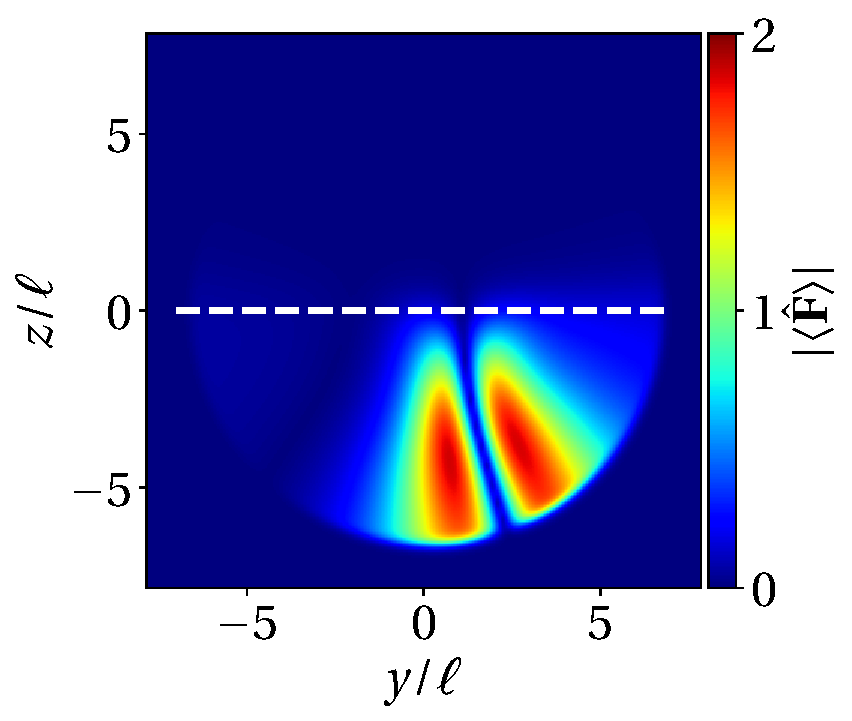
\includegraphics[width=\textwidth]
        {gfx/ch-spin2/UN-BN_VF-SQV_spin_mag.pdf}
        \caption{}
    \end{subfigure}
    \begin{subfigure}{0.45\textwidth}
        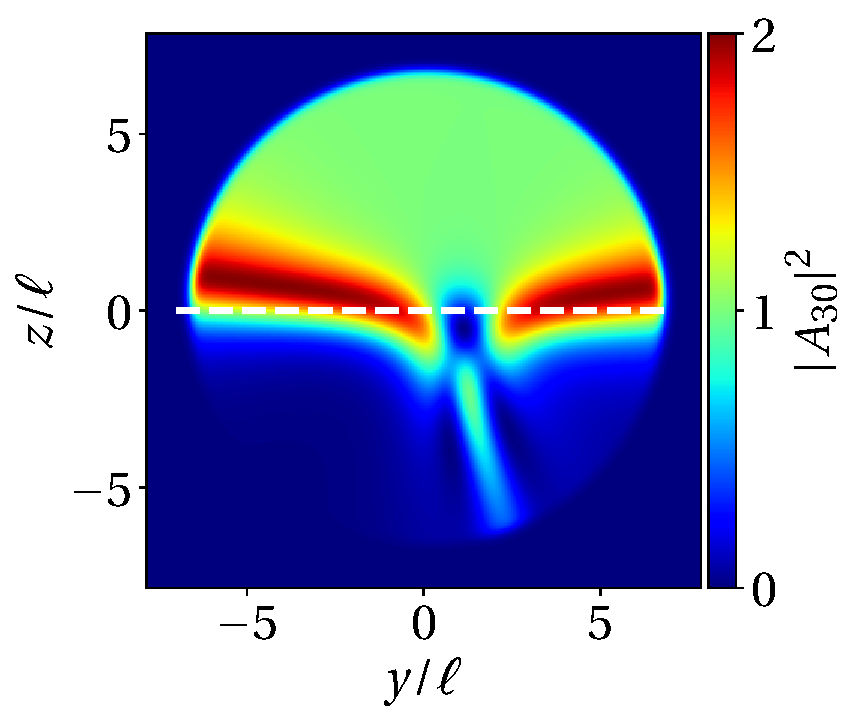
\includegraphics[width=\textwidth]{gfx/ch-spin2/UN-BN_VF-SQV_a30.pdf}
        \caption{}
    \end{subfigure}
    \caption[Dynamics of a singly quantised vortex to vortex-free connection in
    a uniaxial nematic to biaxial nematic interface]
    {\label{fig: UN-BN-VF-SQV} Vortex-free to phase vortex connection defined
    by Eq.~\eqref{eq: UN-BN-SQV-SQV} with \(\beta=0\) and no winding in the
    middle component.
    (a): Spin magnitude at \(\tilde{t}=5\). The HQV cores are identified where
    \(\spinmag = 2\).
    (b): Spin-singlet trio amplitude at \(\tilde{t} = 5\). A cyclic region is
    revealed where \(|A_{30}|^2 = 2\), which arises due to phase differences
    (see Fig~\ref{fig: UN-BN-duo-trio}).}
\end{figure}
The dynamics of this connection closely resembles what the later dynamics of the
BN side of the phase vortex connection would look like, provided that the
vortices were stabilised against leaving the condensate.
We see that the initial phase vortex on the BN side has undergone a splitting
process into two HQVs, each of which can be seen to terminate at the interface.
The cores of the HQVs are easily identified from the
\(\spinmag = 2\) regions.
Similar splitting of a phase vortex into HQVs has been observed in the polar
phase of spin-1 condensates~\cite{Seo2015, Xiao2021}.
For the timescales considered, the resulting HQVs remain stable against
leaving the condensate.
Additionally, we see the clear presence of the cyclic phase emerging at the
interface \(z / \ell \sim 0\), arising due to the phase difference between
the spinor components (see Fig.~\ref{fig: UN-BN-duo-trio}).

\subsection{Cyclic to ferromagnetic interface}
We numerically investigate vortex connections across a topological interface
between the cyclic and \(\text{FM}_2\) phases, given by
Eq.~\eqref{eq: C-FM-interpolating-spinor}.
Since our numerical simulations use parameters that predict a nematic ground
state, we introduce a spatially-dependent \(c_1\) term such that \(c0/c_1=90.7\)
on the cyclic side but \(c_0/c_1=-90.7\) on the FM side, effectively changing
the sign of the \(c_1\) term~\cite{Fatemi2000,Papoular2010}.
Now, in the FM region, the parameters ensure that the FM region remains stable.
Despite the cyclic state not being the predicted ground state, the interface
is observed to remain stable for the timescales considered in our simulations.

We firstly investigate the connection of a third vortex in the cyclic phase
connecting to a singular phase vortex in the \(\text{FM}_2\) phase using
Eq.~\eqref{eq: C-FM-third-pv} as the initial state.
This initial state is then propagated using a short imaginary-time evolution to
imprint the vortex cores and, once the core is imprinted, we switch to
complex-time simulations using a damping coefficient of \(\nu=10^{-2}\).
The resulting spin magnitude and spin-singlet duo amplitude for this interface
after time \(\tilde{t} = 5\) are plotted in Fig.~\ref{fig: C-FM-third-SQV}.
\begin{figure}
    \centering
    \begin{tikzpicture}

        \node[inner sep=0pt] (plot1) at (-5,0)
        {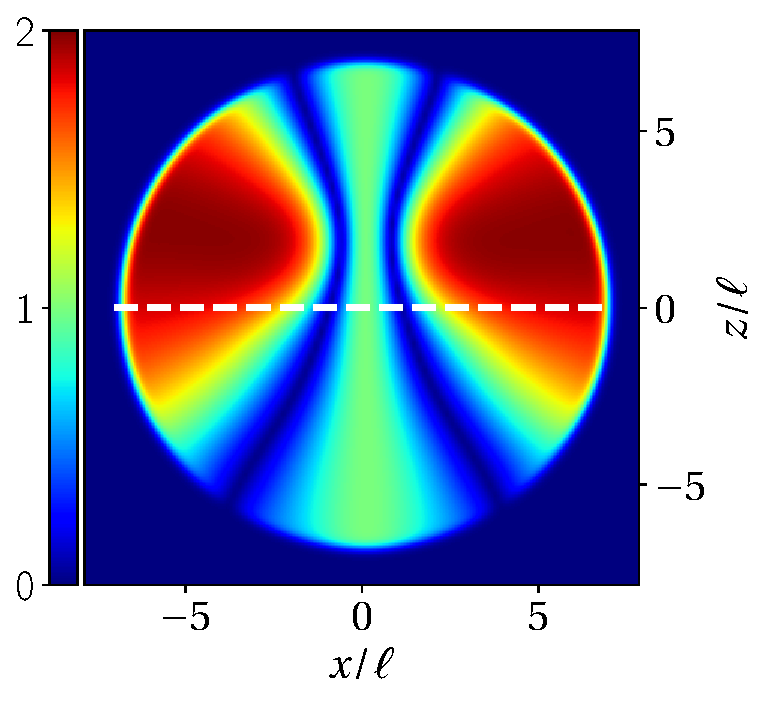
\includegraphics[width=0.33\textwidth]
            {gfx/ch-spin2/C-FM=2_third-SQV_spin_mag.pdf}};
        \node[inner sep=0pt] (plot2) at (-0.6, 0.25)
        {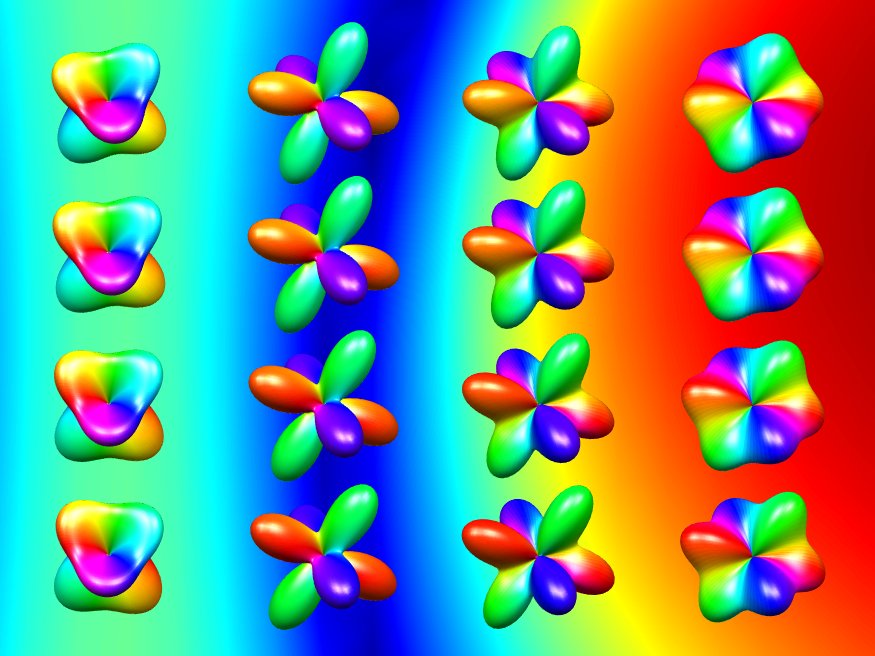
\includegraphics[width=0.25\textwidth, height=0.25\textwidth]
            {gfx/ch-spin2/C-FM=2_third-SQV_spinMag_spherical.pdf}};
        \node[rectangle, draw=black, minimum width=0.5cm, minimum height=0.5cm]
        (rec) at (-4.75, 0.75) {};
        \draw[-, dashed] (rec.north west) -- (plot2.north west) {};
        \draw[-, dashed] (rec.south west) -- (plot2.south west) {};

        \draw[-, thick] (plot2.south east) -- (plot2.north east) {};
        \draw[-, thick] (plot2.south east) -- (plot2.south west) {};
        \draw[-, thick] (plot2.south west) -- (plot2.north west) {};
        \draw[-, thick] (plot2.north west) -- (plot2.north east) {};

        \node[inner sep=0pt] (plot0) at (3.8,0)
        {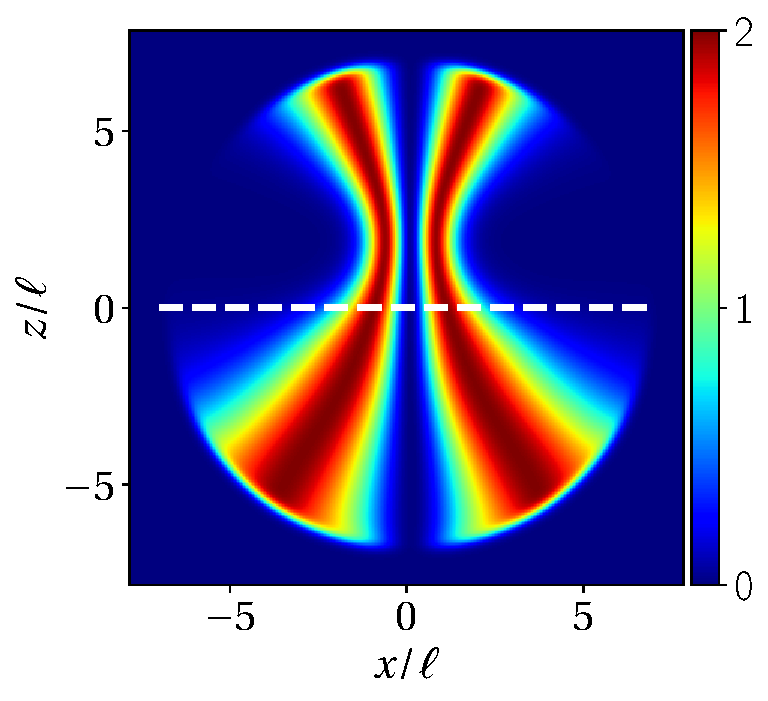
\includegraphics[width=0.33\textwidth]
            {gfx/ch-spin2/C-FM=2_third-SQV_singlet_trio.pdf}};

        % Labels
        \node at (-5.15, -2.5) {(a)};
        \node at (-0.5, -2.5) {(b)};
        \node at (3.95, -2.5) {(c)};
    \end{tikzpicture}
    \caption[Dynamics of a one-third vortex to singly quantised vortex
    connection in a cyclic to ferromagnetic interface]
    {\label{fig: C-FM-third-SQV}One-third vortex to phase vortex connection in
    an interface between the cyclic and \(\text{FM}_2\) phases given by
    Eq.~\eqref{eq: C-FM-third-pv} at \(\tilde{t} = 50\).
    (a): Longitudinal cut of \(\spinmag \) at \(y/\ell=0\).
    The third vortex on the cyclic side (\(z/\ell < 0\)) is evident from the
    \(\spinmag = 1\) core which extends throughout the FM region.
    (b): Zoomed transverse cut of \(\spinmag \) inside the core in the FM
    region.
    Overlaid are the spherical harmonics showing the non-trivial change
    of order parameter symmetry inside the core.
    (c): Longitudinal cut of \(|A_{30}|^2\) at \(y/\ell=0\).
    Cyclic regions are identified from \(|A_{30}|^2=2\).}
\end{figure}
Here, \(\spinmag \) reveals non-trivial core structures emerging.
Clearly one can see the third vortex on the cyclic side of the interface
(\(z/\ell < 0\)) evidenced by the \(\spinmag = 1\) core.
However, unlike the previous case where the vortices spatially separated, this
\(\spinmag = 1\) region then extends throughout the longitudinal extent of the
condensate, and penetrates into the FM region, revealing that the initial phase
vortex of the FM phase has developed a composite core structure.
This composite core structure is separated into three distinct parts:
Inside is the \(\spinmag = 1\) region, which is then encased in a cyclic shell
as seen from the \(|A_{30}|^2=2\) regions in Fig.~\ref{fig: C-FM-third-SQV}c.
Then, far away from the vortex core, the system smoothly interpolates back to
a \(\spinmag = 2\) region in the bulk of the condensate.
The spherical harmonics of the internal core structure plotted in
Fig.~\ref{fig: C-FM-third-SQV}b reveal the non-trivial change of order parameter
symmetry within the composite core.

As we did in the UN to BN case, one can use the general spinor in
Eq.~\eqref{eq: C-FM-third-pv} to analytically predict the vortex core structures
observed when \(\eta \) is a function of the transverse radius
\(\rho = \sqrt{x^2 + y^2}\).
The core can be described by choosing an appropriate function for
\(\eta(\rho)\) that interpolates between all three phases.
In particular, we choose \(\eta(\rho) = 3\tanh(\rho/2) - 1\), which becomes
\(\eta=-1\) (\(\text{FM}_1^-\)) at \(\rho=0\) along the vortex core, \(\eta=0\)
(cyclic) at \(\rho=\tanh^{-1}(1/3)\), and finally \(\eta=2\) (\(\text{FM}_2^+\))
at large \(\rho \).
Thus, this interpolating spinor accurately models the behaviour observed in
Fig.~\ref{fig: C-FM-third-SQV}.

Instead of considering only singular vortices, we can also investigate the
nonsingular vortex connection given in Eq.~\eqref{eq: C-FM-coreless-general}.
We choose this as the initial state, with
\(\beta = \pi\left(1 + \tanh(\rho-1)\right)/2\) to model the required
monotonically increasing function.
Here we focus only on the cyclic to \(\text{FM}_2\) limit, but equivalently the
cyclic to \(\text{FM}_1\) limit can be chosen by an appropriate choice of \(p\)
and \(q\) that interpolates \(\eta \) between \(-1\) and \(0\).
We perform purely imaginary-time simulations to simulate energy relaxation.
\begin{figure}
    \centering
    \begin{tikzpicture}
        % DQV
        \node[inner sep=0pt] (initial_dqv) at (0.4, 0)
        {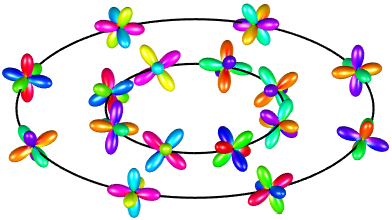
\includegraphics[width=0.3\textwidth]
            {gfx/ch-spin2/C-FM=2_coreless_cyclic_init_spherical.pdf}};
        \node[cylinder, draw, fill=black, opacity=0.5, minimum height=3cm,
            rotate=90] (c_dqv) at (0.4, 0) {};

        % Colour bar
        \node[rotate=90] at (-2.15, 0.2)
        {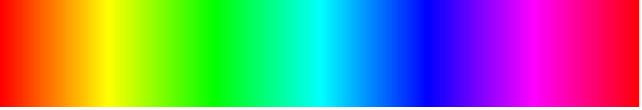
\includegraphics[width=0.15\textwidth, height=0.015\textheight]
            {gfx/colourbars/hsv_colourbar.pdf}};
        \node[rotate=90] at (-2.15, -1.8) {Arg(\(Z\)) = 0};
        \node[rotate=90] at (-2.15, 1.7) {\(2\pi \)};

        % Spin mag
        \node[inner sep=0pt] (spinmag_dqv) at (5, 0)
        {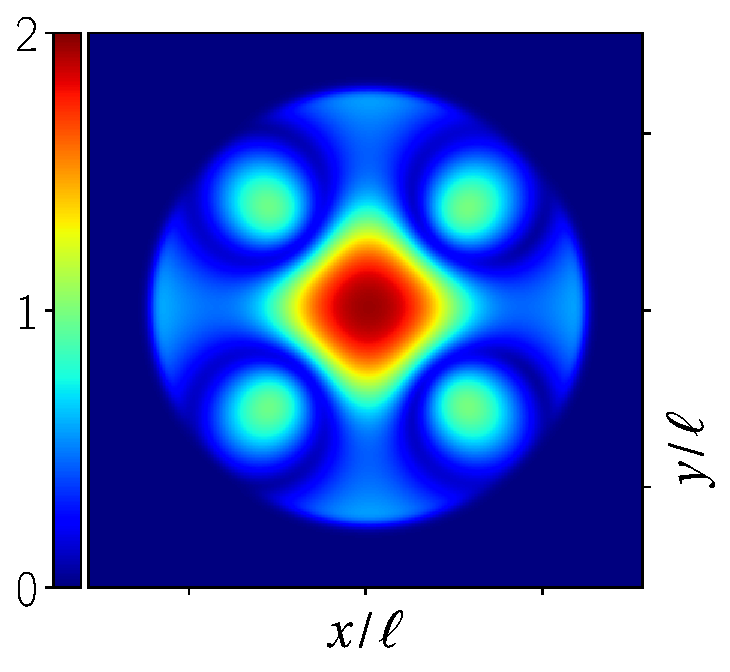
\includegraphics[width=0.3\textwidth]
            {gfx/ch-spin2/C-FM=2_coreless_cyclic_spin_mag.pdf}};

        % Third spherical
        \node[inner sep=0pt] (third_spherical) at (10, 1.5)
        {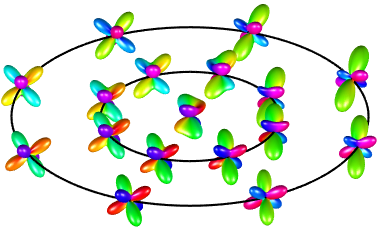
\includegraphics[width=0.3\textwidth]
            {gfx/ch-spin2/C-FM=2_coreless_cyclic_third_spherical.pdf}};
        \node[cylinder, draw, fill=green, opacity=0.5, minimum height=2.8cm,
            rotate=90] (c_third) at (10, 1.5) {};
        \node[rectangle, draw, minimum width=0.3cm, minimum height=0.3cm,
            dashed, green]
        (third_small_rec) at (5.8, 0.6) {};
        \node[rectangle, draw, minimum width=4.4cm, minimum height=2.9cm,
            green] (third_big_rec) at (10, 1.6) {};
        \draw[-, dashed, green]
        (third_big_rec.north west) -- (third_small_rec.north west) {};
        \draw[-, dashed, green]
        (third_big_rec.south west) -- (third_small_rec.south east) {};

        % Two-third spherical
        \node[inner sep=0pt] (third_spherical) at (10, -1.5)
        {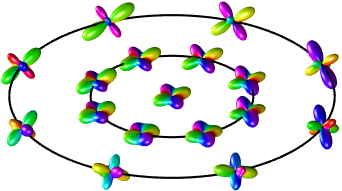
\includegraphics[width=0.3\textwidth]
            {gfx/ch-spin2/C-FM=2_coreless_cyclic_2third_spherical.pdf}};
        \node[cylinder, draw, fill=red, opacity=0.5, minimum height=2.8cm,
            rotate=90] (c_2third) at (10, -1.5) {};
        \node[rectangle, draw, dashed, minimum width=0.7cm,
            minimum height=0.7cm, rotate=45, opacity=0.5, red]
        (2third_small_rec) at (5.35, 0.15) {};
        \node[rectangle, draw, minimum width=4.4cm, minimum height=2.9cm,
            red] (2third_big_rec) at (10, -1.4) {};
        \draw[-, dashed, red]
        (2third_big_rec.north west) -- (2third_small_rec.south east) {};
        \draw[-, dashed, red]
        (2third_big_rec.south west) -- (2third_small_rec.south west) {};

        % Labels
        \node at (0.4, -2.3) {(a)};
        \node at (5, -2.3) {(b)};
        \node at (8.2, 2.7) {(c)};
        \node at (8.2, -0.3) {(d)};
    \end{tikzpicture}
    \caption[Dynamics of the doubly quantised vortex connection in a cyclic to a
        ferromagnetic interface]
    {\label{fig: C-FM-coreless-cyclic}Schematic representation of the
        splitting process occurring on the cyclic side of the interface
        (\(z/\ell < 0\)) given by the state in
        Eq.~\eqref{eq: C-FM-coreless-general}.
        (a): Spherical harmonic representation of the initial doubly quantised
        vortex line. By traversing a point about the vortex line, the condensate
        phase is seen to wind by \(4\pi \).
        (b) Transverse cut of \(\spinmag \) at \(z/\ell \approx -3\) after
        imaginary-time evolution at \(\tilde{t} = 1.5\) showing the splitting of
        the initial doubly quantised vortex into fractional vortices.
        The one-third and two-third vortices are clearly identified from the
        \(\spinmag = 1\) and \(\spinmag = 2\) regions, respectively.
        (c) and (d): Spherical harmonic representations about the one-third and
        two-third vortices, respectively.
        The spherical harmonics shows the non-trivial change of the order
        parameter symmetry as we move away from the vortex cores.}
\end{figure}
We start by discussing the dynamics of the doubly quantised vortex on the cyclic
side of the interface, shown in Fig.~\ref{fig: C-FM-coreless-cyclic}.
As expected for a doubly quantised vortex line, it very rapidly undergoes a
splitting process.
In this case, it splits into four one-third vortices, evidenced by the
\(\spinmag = 1\) regions, and a further two-third vortex, evidence by the large
\(\spinmag = 2\) region.
The discrepancy of the core size could arise from the different vortices being
set by different healing lengths.
Analysis of the spherical harmonics in Fig.~\ref{fig: C-FM-coreless-cyclic}c,d
shows the non-trivial order parameter symmetry both within and outside the
vortex cores.
By following the spherical harmonics about the vortex cores, the condensate
phase changes by \(2\pi/3\) and \(4\pi/3\) confirming that these structures are
one-third and two-third vortices.
Due to the energy relaxation, the one-third vortices quickly leave the
condensate.
However, the two-third vortex is first observed to undergo a further splitting
process in which it splits into two one-third vortices, which then proceed to
exit the condensate cloud.

The initial nonsingular vortex on the FM side of the interface also undergoes a
complex splitting process, shown in Fig.~\ref{fig: C-FM-coreless-FM}.
\begin{figure}
    \centering
    \begin{tikzpicture}
        % Colour bar
        \node[rotate=90] at (9, 0)
        {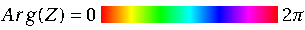
\includegraphics{gfx/colourbars/compiled_hsv.pdf}};

        % Spin mag
        \node[inner sep=0pt] (spinmag_coreless) at (-2, 0)
        {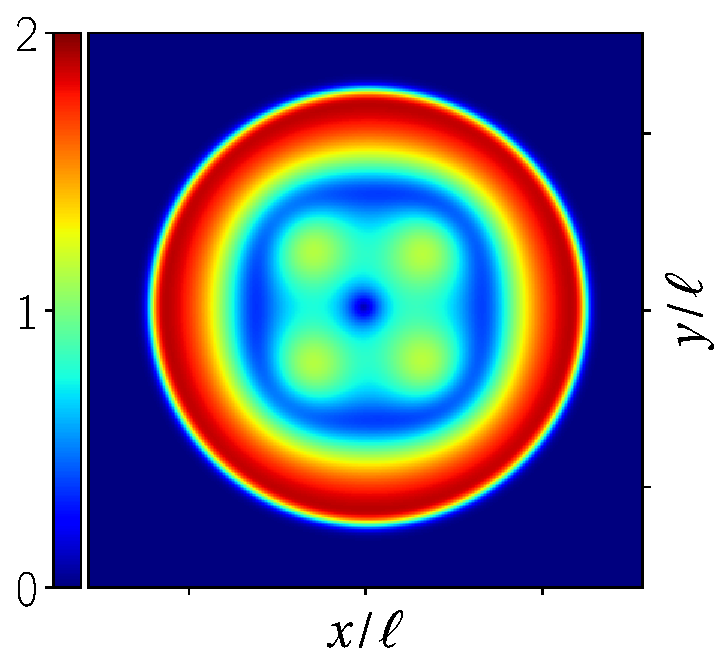
\includegraphics[width=0.45\textwidth]
            {gfx/ch-spin2/C-FM=2_coreless_FM_spin_mag.pdf}};

        % After splitting
        \node[inner sep=0pt] (initial_dqv) at (5, 0.2)
        {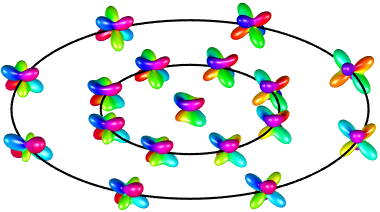
\includegraphics[width=0.45\textwidth]
            {gfx/ch-spin2/C-FM=2_coreless_FM_after_spherical.pdf}};

        \node[rectangle, draw, minimum width=0.5cm, minimum height=0.5cm]
        (small_rec) at (-1.9, -0.12) {};
        \node[rectangle, draw, minimum width=6.6cm, minimum height=3.7cm]
        (big_rec) at (5, 0.2) {};
        \draw[-, dashed] (big_rec.north west) -- (small_rec.north east) {};
        \draw[-, dashed] (big_rec.south west) -- (small_rec.south east) {};

        % Labels
        \node at (-2.25, -3) {(a)};
        \node at (5, -3) {(b)};
    \end{tikzpicture}
    \caption[Dynamics of a nonsingular vortex connected across a cyclic to
        ferromagnetic interface]
    {\label{fig: C-FM-coreless-FM}Schematic representation of the
        splitting process occurring on the FM side of the interface
        (\(z/\ell > 0\)) of the state in Eq.~\eqref{eq: C-FM-coreless-general}.
        The initial state on this side of the interface is given explicitly in
        Eq.~\eqref{eq: FM-2-coreless} with Euler angles given in
        Eq.~\eqref{eq: coreless-euler-limits-FM-2}.
        (a) Transverse cut of \(\spinmag \) at \(z/\ell \approx 3\) after
        complex-time evolution at \(\tilde{t} = 1.5\).
        The singular vortex structures can be seen from the
        \(\spinmag \approx 1\) cores.
        (b): Spherical harmonic representation of the internal structure of
        the singular vortex, showing the non-trivial symmetry within the core.}
\end{figure}
The nonsingular vortex is observed to split into four singular vortices,
observed from transverse cuts of \(\spinmag \).
Analysis of the spherical harmonics reveal the non-trivial symmetry within
the singular vortex cores.
As in the case on the cyclic side, these vortices rapidly leave the condensate
due to the energy relaxation.
On both sides of the interface the vortex structures are observed to terminate
at the interface itself, and do not connect in a way that is observed in the
phase vortex to one-third vortex connection (see
Fig.~\ref{fig: C-FM-third-SQV}).

\section{Conclusions}
In this chapter we have presented spin-2 BECs as a medium for investigating
topological interface physics.
We constructed topological interfaces within the condensate by means of
interpolating spinor wave functions which are derived from steady-state
solutions to the spin-2 GPEs, which smoothly connect different phases using
an interpolation parameter.
In each case we constructed multiple different classes of topological defects
which either connected smoothly across the interface, or terminated on the
interface itself.
In particular, we showed how phase, spin, and fractional vortices could be
constructed simply from the component phase windings, and how more complicated
connections could be constructed by applying a spin rotation to the general
interface spinor with appropriate choices for the Euler angles.
It was shown that interfaces between the nematic phases allow for monopoles and
nonsingular vortices on one side of the interface to smoothly connect to
singular line defects on the other side.
In addition, interfaces involving the FM phases can be engineered to contain
a generalisation of the Dirac monopole in the FM limit, which connects to a
singular vortex line in the opposite limit.

Numerical investigations of the UN to BN and cyclic to FM interfaces were also
performed.
We showed that phase vortices in a UN to BN interface had two distinct parts to
their dynamics.
The initially overlapping vortex lines quickly spatially separated, arising from
an instability at the interface itself.
Each vortex then developed composite core structures that contained UN, BN, and
cyclic phases, forming a topological interface within the vortex cores
themselves.
A phase vortex in the BN phase terminating at the interface was also
investigated, which was observed to split into a pair of HQVs with FM cores,
which also terminated at the interface.
In the cyclic to FM interface, we observed a phase vortex in the FM phase
smoothly connect to a one-third vortex in the cyclic limit by forming a
composite structure that had an inner \(\spinmag=1\) core, encased by a
surrounding cyclic region, before smoothly interpolating back to the
\(\spinmag=2\) bulk.
Lastly, a connection involving a nonsingular vortex was numerically simulated.
We showed that the initial nonsingular structure on the FM side connected
smoothly to a doubly quantised phase vortex in the cyclic limit.
The nonsingular vortex was then observed to split into four singular structures,
whilst the doubly quantised phase vortex split into four one-third vortices,
with a large two-third vortex in the centre of the condensate.